%
% hyperbolic.tex -- XXX
%
% (c) 2008 Prof Dr Andreas Mueller
% $Id: c06-hyperbolisch.tex,v 1.3 2008/10/31 08:04:16 afm Exp $
%
\chapter{Hyperbolische Differentialgleichungen\label{chapter-hyperbolisch}}
\index{Differentialgleichung!partielle!hyperbolische}
\index{Wellengleichung}
\lhead{Hyperbolische PDGL}
\rhead{}
In diesem Kapitel wird als prominentes Beispiel einer hyperbolischen
Differentialgleichung die Wellengleichung diskutiert.
Wie im parabolischen Fall hat die Zeitkoordinate eine spezielle Bedeutung,
auch die Wellengleichung ist eine ``Zeitentwicklungsgleichung'', allerdings
zweiter Ordnung. Während sich eine Änderung der Anfangs- oder Randbedingung
bei einem elliptischen Problem sofort überall auf die Lösung auswirkt,
breiten sich solche Änderungen bei der Wellengleichung mit endlicher
Geschwindigkeit aus. Zu jedem Punkt gibt es also Punkte, auf die sich eine
Wertänderung auswirken kann, und andere, die davon nichts mitbekommen.
Die Grenzflächen zwischen diesen Bereichen sind eine wichtige Grundlage
für das Verständnis der Lösungen.

Zunächst werden daher die Lösungen 
am eindimensionalen Fall bestimmt und die in beide Richtungen laufenden 
Wellenlösungen demonstriert. Diese geben Anlass zu einer Untersuchung,
zu welcher Art von Anfangsbedingung die Wellengleichung überhaupt
lösbar ist. Dies führt uns dann auf den Begriff der Charakteristiken.

%
% c02-separation.tex
%
% (c) 2008 Prof Dr Andreas Mueller
% $Id: c02-separation.tex,v 1.3 2008/09/13 23:01:45 afm Exp $
%
\lhead{Separation der Variablen}
\rhead{}
\chapter{Separation der Variablen\label{chapter-separation}}
\index{Stroboskop}
\index{Eigenschwingung}
\index{stehende Welle}
\begin{figure}
\begin{center}
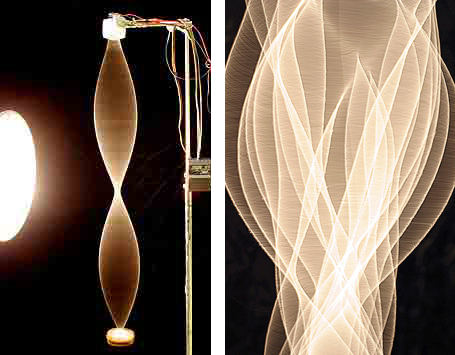
\includegraphics[width=0.8\hsize]{graphics/stringvibrlarge-10-06-06.jpg}
\end{center}
\caption{Schwingende Saite (Bild von A.~Davidhazy, http://people.rit.edu/andpph/)
\label{separation:schwingendesaite}}
\end{figure}
Beleuchtet man eine schwingende Saite mit einem Stroboskop mit der
Frequenz der Eigenschwingung, scheint die Saite stillzustehen. 
In periodischen Zeit\-ab\-st"an\-den sieht die L"osung der Wellengleichung
also gleich aus.
Misst man andererseits die Auslenkung der Saite
an einer Stelle in Abh"angigkeit von der Zeit, beobachtet man
eine harmonische Schwingung, die sich mit Hilfe von $\sin$- und
$\cos$-Funktionen beschreiben l"asst. Man kann also vermuten,
dass die L"osung der Wellengleichung der schwingenden Saite
ein Produkt
\[
u(x,t)=X(x)\cdot\sin\omega t\quad\text{oder}\quad X(x)\cdot\cos\omega t.
\]
ist. Ziel dieses Kapitels ist, diese Idee zu einem L"osungsverfahren
weiterzuentwickeln und auf einige Differentialgleichungen anzuwenden.

\section{Separation der Variablen f"ur gew"ohnliche Differentialgleichungen}
Die Differentialgleichung 
\begin{equation}
y'-xy=0
\label{separation:ode}
\end{equation}
kann mit Separation der Variablen gel"ost werden:
\begin{align*}
\frac{dy}{dx}&=xy\\
\frac1y\,dy&=x\,dx\\
\int\frac1y\,dy&=\int x\,dx\\
\log|y|&=\frac12x^2+C\\
y&=y_0e^{\frac12x^2}
\end{align*}
Das Verfahren beruht auf dem Prinzip, auf jeder Seite der Gleichung
nur eine Variable zu haben.
Dabei zerlegt man sogar die Ableitung $dy/dx$, was man ja eigentlich
gar nicht darf.
Die Separation f"uhrt die L"osung der Differentialgleichung auf die
Berechnung zweier Integrale zur"uck, also eigentlich auf die
L"osung einer besonders einfachen Differentialgleichung der Form $y'=f(x)$
mit L"osung $y(x)=\int f(x)\,dx$.
Diese Form der L"osung sagt uns auch genau, was wir an Anfangsbedingungen
brauchen.
Ist $y_0$ der Wert der L"osung an der Stelle $x_0$, dann liefert
das Integral die L"osungsfunktion
\[
y(x)=\int_{x_0}^xf(\xi)\,d\xi + y_0.
\]

So einfach wird es f"ur partielle Differentialgleichungen nicht sein.
Insbesondere f"ur die an sich schon etwas ``anr"uchige'' Operationen,
den Differentialquotienten $dy/dx$ auseinanderzureissen gibt es keinerlei
Entsprechung bei partiellen Ableitungen.
Unter geeigneten Voraussetzungen an das Gebiet und die Differentialgleichung
ist es aber immer noch denkbar, dass man die Variablen trennen kann,
also 
\[
\text{Funktionen/Ableitungen nur mit $x$} = \text{Funktionen/Ableitungen nur mit $y$}
\]
Da die linke Seite nur von $x$ abh"angt, die rechte aber nur von $y$, m"ussen
beide Seiten konstant sein, die partielle Differentialgleichung zerf"allt
in eine linke {\em gew"ohnliche} Differentialgleichung f"ur eine Funktion von
$x$ und eine rechte {\em gew"ohnliche} Differentialgleichung f"ur $y$.

Da wir "uber gew"ohnliche Differntialgleichungen Bescheid wissen, sollte
es uns so m"oglich sein, eine partielle Differentialgleichung zu l"osen
und herzuleiten, welche Art von Randwerten vorgegeben werden m"ussen, damit
die Differentialgleichung eindeutig l"osbar ist.

\section{Idee des Verfahrens}
Oft hat man aus dem Anwendungsgebiet, aus dem eine partielle
Differentialgleichung stammt, Hinweise darauf, wie die L"osungsfunktion
von {\em einer} der unabh"angigen Variablen abh"angt.
Dann kann man Versuchen, die L"osung als Produkt oder Summe von
solchen ``vermuteten'' Funktionen darzustellen.

\index{Ansatz}
\index{Separationsansatz}
Aber selbst wenn man nichts "uber die L"osung weiss, kann man 
versuchen, die L"osung als Summe oder Produkt von Funktionen darzustellen,
die nur von jeweils einer Variablen abh"angen. Als Beispiel versuchen
wir die lineare Differentialgleichung 
\begin{equation}
\frac1x
\frac{\partial u}{\partial x}
+
\frac1y
\frac{\partial u}{\partial y}
=\frac1{y^2}
,
\qquad x>1, y>1
\label{separation:beispiel1}
\end{equation}
zu l"osen, wobei wir die Randbedingungen f"ur den Moment ignorieren.
Wir versuchen, die L"osung als Summe von zwei Funktionen darzustellen,
welche nur von $x$ bzw.~$y$ abh"angen, also
\begin{equation}
u(x,y)=X(x)+Y(y)
\quad\Rightarrow\quad
\begin{cases}
\quad{\displaystyle \frac{\partial u}{\partial x}}&=X'(x)\\
\\
\quad{\displaystyle \frac{\partial u}{\partial y}}&=Y'(y)\\
\end{cases}
\label{separation:beispiel1:ansatz}
\end{equation}
Setzt man dies in die Differentialgleichung (\ref{separation:beispiel1})
ein, erhalten wir die Gleichung
\[
\frac{X'(x)}{x}+\frac{Y'(y)}{y}=\frac1{y^2}
\]
oder
\begin{equation}
\frac{X'(x)}{x}
=\frac1{y^2}
-\frac{Y'(y)}{y}.
\label{separation:beispiel1:separiert}
\end{equation}
Die Form (\ref{separation:beispiel1:separiert}) hat eine besondere
Eigenschaft: die Variable $x$ kommt nur auf der linken Seite vor,
die Variable $y$ nur auf der rechten. Setzt man f"ur $y$ irgend
einen Wert ein, ver"andert sich die rechte Seite nicht mehr,
die linke Seite muss also f"ur alle $x$ den gleichen Wert geben.
L"asst man jetzt wieder das $y$ varieren, muss sich auch auf der rechten
Seite immer der gleiche Wert ergeben. Wir nennen den gemeinsamen Wert
$k$, und bekommen zwei gew"ohnliche Differentialgleichungen
f"ur $X(x)$ und $Y(y)$:
\begin{align}
\frac{X'(x)}{x}&=k
&
k&=\frac1{y^2}-\frac{Y'(y)}{y}
\label{separation:beispiel1:separiertedgl}
\end{align}
Die linke Differentialgleichung ist einfach zu l"osen:
\begin{align*}
X'(x)&=kx\quad\Rightarrow\quad X(x)=
\frac12kx^2+C_x.
\end{align*}
Die rechte Differentialgleichung ist nur leicht komplizierter:
\begin{align*}
Y'(y)=\frac1y-ky
\quad\Rightarrow\quad
Y(y)=\int\frac1y-ky\,dy=
\log y-\frac12ky^2+C_y.
\end{align*}
Diese beiden L"osungen k"onnen wir jetzt wieder zu einer L"osung der
urspr"unglichen Differentialgleichung zusammensetzen:
\begin{equation}
u(x,y)=
\frac12kx^2+
\log y-\frac12ky^2+C.
\label{separation:beispiel1:loesung}
\end{equation}
Wir haben damit eine unendliche Familie von L"osungen der
Differentialgleichung gefunden, f"ur jedes Paar $(k,C)$ von
Parametern liefert die Formel (\ref{separation:beispiel1:loesung})
eine L"osung.
Dazu m"ussen wir in irgend einer Weise die Randbedingungen verwenden.
Damit haben wir eine Skizze f"ur das L"osungsverfahren mit Separation:
\begin{enumerate}
\item Finde einen L"osungsansatz aus Funktionen, die nur von einer
Variablen abh"angen.
\item Setze in die Differentialgleichung ein und separiere die Terme
so, dass zwei Variablen jeweils nur auf einer Seite vorkommen. Dann
h"angen beide Seiten nicht mehr von dieser Variablen ab, jede Seite
ist eine Differentialgleichung mit weniger Variablen.
\item L"ose die Teildifferentialgleichungen, und setze daraus 
L"osungen zusammen. 
\item Verwende die Randbedingungen, um eine L"osung zu finden.
\end{enumerate}
Wie man unschwer erkennen kann, ist weniger die L"osung der
einzelnen Teildifferentialgleichungen das Problem, sondern der letzte
Schritt. In den folgenden Abschnitten zeigen wir an Beispielen, wie
dies m"oglich ist.

\section{Separation f"ur lineare partielle Differentialgleichungen}
Die Grundidee des Separationsverfahrens liefert eine Familie von Funktionen,
von ein paar Integrationskonstanten abh"angen. Vorgegeben sind auf dem
Rand aber beliebige Funktionen, es ist im Allgemeinen nicht m"oglich,
durch richtige Wahl von wenigen Parametern beliebige Funktionen zu erhalten.
Des Separationsverfahren in der bisherigen Form kann also ein
beliebiges Randwertproblem noch nicht l"osen.

Nehmen wir an, es m"usse die Differentialgleichung $Lu=f$ auf dem
Gebiet $\Omega$ mit Randwerte $g(x)$ f"ur $x\in\partial \Omega$
gel"ost werden.
Wir haben nur dann eine Chance, aus den bisherigen Resultaten eine 
vollst"andige L"osung des Problems zu erhalten, wenn wir in der
Lage sind, solche Teill"osungen zu einer vollst"andigen L"osung
zu kombinieren. Dazu sind aber im allgemeinen zus"atzliche
Bedingungen an die Differentialgleichung n"otig. Linearit"at der
Differentialgleichung ist, was wir hier verwenden wollen:

\begin{satz}Sind $u_1$ und $u_2$ L"osungen einer homogenen linearen partiellen
Differentialgleichung, dann sind auch $u_1+u_2$ und $\lambda u_1$ f"ur
$\lambda\in\mathbb R$ L"osungen
\end{satz}

\begin{proof}[Beweis]
Die Differentialgleichung
\[
F(x_1,\dots,x_2,u,\frac{\partial u}{\partial x_1},\dots)=0
\]
ist linear in $u$ und den Ableitungen, man darf also Summen und Vielfache
in $u$ und den Ableitungen aus der Funktion herausziehen:
\begin{align*}
F(x_1,\dots,x_2,u_1+u_2,\frac{\partial u_1}{\partial x_1}+\frac{\partial u_2}{\partial x_1},\dots)
&=
F(x_1,\dots,x_2,u_1,\frac{\partial u_1}{\partial x_1},\dots)
\\
&+
F(x_1,\dots,x_2,u_2,\frac{\partial u_2}{\partial x_1},\dots)=0
\\
F(x_1,\dots,x_2,\lambda u_1,\frac{\partial \lambda u_1}{\partial x_1},\dots)
&=
\lambda
F(x_1,\dots,x_2,u_1,\frac{\partial u_1}{\partial x_1},\dots)
=0
\end{align*}
Die Linearkombinationen von $u_1$ und $u_2$ sind also auch L"osungen.
\end{proof}

Um die Differentialgleichung zu l"osen, kann man also versuchen, mit
dem bisherigen Separationsverfahren m"oglichst viele L"osungen zu
$u_1$, $u_2$, $u_3,\dots$ zu finden, und diese dann zu einer Gesamtl"osung
zu kombinieren
\[
u(x)=\sum_{i=1}^\infty a_ku_k
\]
mit geeigneten Koeffizienten $a_k$, die so zu w"ahlen sind, dass die
Randbedingungen erf"ullt sind.

Inhomogene lineare partielle Differentialgleichungen kann man mit diesem
Verfahren ebenfalls l"osen. Dazu findet man zun"achst eine partikul"are
L"osung $u_p$, welche die inhomogenen Differentialgleichung l"ost, ohne
allerdings korrekte Randwerte zu liefern.
Das urspr"ungliche Separationsverfahren kann hierbei hilfreich sein.
Dann verwendet man das skizzierte Verfahren f"ur homogene lineare
partielle Differentialgleichungen f"ur modifizierte Randwerte $g-u_p$ auf
$\partial\Omega$ um eine L"osung der homogenen Gleichung $u_h$ zu finden.
Die Summe $u=u_p+u_h$ ist dann eine L"osung der inhomogenen Gleichung
mit Randwerten $u_p + (g-u_p)=g$, also ein L"osung des urspr"unglichen
Problems.

Die Bestimmung der Koeffizienten $a_k$ f"ur die gefundene Familie
von Teill"osungen f"uhrt oft auf die Fourier-Theorie, oder allgemeiner
auf orthogonale Funktionenfamilien. Solche Teill"osungen haben oft eine
unmittelbare physikalische Bedeutung, zum Beispiel treten sie auf als
Schiwngungsmoden (in der Mechanik oder Elektrotechnik) oder als
Elektronenzust"ande in der Quantenmechanik.

\section{Schwingende rechteckige Membran}
\rhead{Rechteckige Membran}
\index{Membran!rechteckig}
Wir betrachten die Schwingung einer rechteckigen Membran, die am Rande
des Gebietes
\[
R=\{(x,y)\,|\,0\le x\le a,0\le y\le b\} =(0,a)\times(0,b)
\]
eingespannt ist. Zur Zeit $t=0$ sei die Form der Membran durch die
Funktion $f(x,y)$ gegeben.
F"ur beliebige Zeit $t\ge 0$ wird sie beschrieben durch eine Funktion $u(x,y,t)$,
welche der Differentialgleichung
\[
\frac1{c^2}\frac{\partial^2u}{\partial t^2}=\frac{\partial^2u}{\partial x^2}+\frac{\partial^2u}{\partial y^2}
\]
gen"ugt mit den Anfangsbedingungen
\begin{align*}
u(x,y,0)&=f(x,y)\quad\forall 0\le x\le a,0\le y\le b,
\\
\frac{\partial}{\partial t}u(x,y,0)&=g(x,y)\quad\forall 0\le x\le a,0\le y\le b
\end{align*}
und den Randbedingungen
\begin{align*}
u(0,y,t)&=0&u(a,y,t)&=0&\forall t\ge 0,0\le y\le b,\\
u(x,0,t)&=0&u(x,b,t)&=0&\forall t\ge 0,0\le x\le a.
\end{align*}

\subsection{Separation der Zeit}
\index{Separation}
Nach der in der Einleitung motivierten Idee suchen wir L"osungen also
Produkt einer Funktion $T(t)$, die nur von der Zeit abh"angt, und einer Funktion
$\varphi(x,y)$, welche nur vom Ort abh"angt, also
\[
u(x,y,t)=T(t)\cdot\varphi(x,y).
\]
Leider kann ein einzelnes solches Produkt nicht alle Anfangsbedingungen
erf"ullen. W"are dies n"amlich m"oglich, m"usste $\varphi(x,y)\sim f(x,y)$
sein und alle Teile der Membran w"urden im Gleichtakt hin und her schwingen.
Simulationen oder physikalische Experimente zeigen aber, dass es
Anfangsbedingungen gibt, bei denen die Teile der Membran gegenl"aufig
schwingen.

Anderseits, muss die L"osung auf jeden Fall die Randbedingung erf"ullen,
es muss also gelten
\begin{align*}
\varphi(0,y)&=0&\varphi(a,y)&=0&0\le y\le b\\
\varphi(x,0)&=0&\varphi(x,b)&=0&0\le x\le a
\end{align*}
Setzen wir diesen Ansatz f"ur $u$ in der Wellengleichung ein,
erhalten wir
\[
\frac1{c^2}T''(t)\varphi(x,y)=T(t)\left(
\frac{\partial^2\varphi}{\partial x^2}
+
\frac{\partial^2\varphi}{\partial y^2}
\right)
\]
Wir suchen eine Funktion $u$, die nicht identisch verschwindet,
es gibt also einige Zeitpunkte $t$ und Orte $(x,y)$, an denen $T(t)$
und $\varphi(x,y)$ nicht verschwinden. An diesen Stellen kann man die
Gleichung umformen in
\begin{equation}
\frac1{c^2}\frac{T''(t)}{T(t)}
= \frac1{\varphi(x,y)}\left( \frac{\partial^2\varphi}{\partial x^2}
+ \frac{\partial^2\varphi}{\partial y^2} \right)
\label{separiertMembran}
\end{equation}
Die rechte Seite h"angt nur
vom Ort ab, darf sich also nicht "andern, wenn man die Zeit $t$ variert.
Als Funktion der Zeit muss die linke Seite eine Konstante sein,
es gibt also ein $k$ mit der Eigenschaft
\[
\frac1{c^2}\frac{T''(t)}{T(t)}=k
\qquad\Leftrightarrow\qquad
T''(t)=k T(t).
\]
Diese gew"ohnliche Differentialgleichung hat L"osungen der Form 
$e^{\pm\sqrt{k}t}$ f"ur positives $k$. F"ur negatives $k$ sind $\sin\sqrt{k}t$ 
und $\cos\sqrt{k}t$ L"osungen.
Aus physikalischer Sicht sind nur L"osungen mit Schwingungscharakter sinnvoll,
wir k"onnen daher annehmen, dass $k<0$.
Ein solches $k$ l"asst sich in der Form $k=-\lambda^2$ schreiben.
Es gibt also ein $\lambda$ mit der Eigenschaft
\[
\frac1{c^2}\frac{T''(t)}{T(t)}=-\lambda^2
\]
oder
\[
T''(t)=-c^2\lambda^2 T(t).
\]
Dies ist eine gew"ohnliche Differentialgleichung zweiter Ordnung, welche mit
bekannten Methoden gel"ost werden kann.
Die allgemeine L"osung dieser Gleichung ist von der Form
\[
A\cos c\lambda t+B\sin c\lambda t.
\]

\subsection{Reduktion auf ein Eigenwertproblem}
\index{Eigenwertproblem}
Die linke Seite von (\ref{separiertMembran}) h"angt nur von der Zeit ab, darf sich
also nicht "andern, wenn man $x$ oder $y$ variert. Als Funktion des Ortes
muss die rechte Seite also ebenfalls konstant sein:
\begin{align*}
\frac1{\varphi(x,y)}\left(
\frac{\partial^2\varphi}{\partial x^2}
+
\frac{\partial^2\varphi}{\partial y^2}
\right)&=-\lambda^2\\
\frac{\partial^2\varphi}{\partial x^2}
+
\frac{\partial^2\varphi}{\partial y^2}
=\Delta\varphi
&=-\lambda^2
\varphi(x,y)
\end{align*}
Die gesuchte Funktion $\varphi$ ist also ein Eigenvektor des linearen
Operators $\Delta$ zum Eigenwert $-\lambda^2$.
Nur die Eigenwerte des Operator $\Delta$ kommen also f"ur die
Zeitabh"angigkeitsgleichung in Frage.

\subsection{Separation von $x$ und $y$}
\index{Separation}
F"ur das Eigenwertproblem k"onnen wir erneut den Separationsansatz
\[
\varphi(x,y)=X(x)\cdot Y(y)
\]
versuchen.
Einsetzen in die Differentialgleichung ergibt
\begin{align*}
X''(x)Y(x)+X(x)Y''(y)&=-\lambda^2 X(x)Y(y)
\\
\frac{X''(x)}{X(x)}+\frac{Y''(y)}{Y(y)}&=-\lambda^2
\end{align*}
Jeder der Br"uche h"angt nur von jeweils einer Variable ab, was nur
m"oglich ist, wenn beide Terme konstant sind. Damit ist das Problem
reduziert auf zwei Gleichungen
\begin{align*}
X''(x)&=-\lambda_1^2X(x)\\
Y''(y)&=-\lambda_2^2Y(y)\\
\lambda_1^2+\lambda_2^2&=\lambda^2
\end{align*}
Die allgemeinen L"osungen dieser Gleichungen, die auch die Randbedingung
bei $x=0$ bzw.~$y=0$ erf"ullt, sind
\begin{align*}
X(x)&=A\sin \lambda_1x\\
Y(y)&=B\sin \lambda_2y
\end{align*}
Die Randbedingungen f"ur $x=a$ und $y=b$ k"onnen nur erf"ullt werden,
wenn $\lambda_1a$ und $\lambda_2b$ Vielfache von $\pi$ sind, also
\[
\lambda_1=\frac{k\pi}a
\qquad
\text{und}
\qquad
\lambda_2=\frac{l\pi}b
\]
Die m"oglichen Werte von $\lambda$ sind also
\[
\lambda_{kl}^2=\left(\frac{k^2}{a^2} + \frac{l^2}{b^2}\right)\pi^2,\qquad k,l\in\mathbb Z
\]
Damit kann man jetzt die allgemeine L"osung des Schwingungsproblems aus den
Teill"osungen
\[
\varphi_{kl}(x,y)=\sin \frac{k\pi}{a}x\sin\frac{l\pi}{b}y
\]
f"ur das Eigenwertproblem
und den Teill"osungen
\[
u_{kl}(x,y,t)
=
(A_{kl}\cos c\lambda_{kl} t+
B_{kl}\sin c\lambda_{kl} t)
\sin \frac{k\pi}{a}x\sin\frac{l\pi}{b}y
\]
f"ur das zeitabh"angige Problem
zu einer allgemeinen L"osung
\begin{equation}
u(x,y,t)=\sum_{k,l}
(A_{kl}\cos c\lambda_{kl} t+
B_{kl}\sin c\lambda_{kl} t)
\sin \frac{k\pi}{a}x\sin\frac{l\pi}{b}y
\label{allgemeineloesung}
\end{equation}
zusammensetzen.

\subsection{Anfangsbedingungen}
\index{Anfangsbedingungen}
Die allgemeine L"osung muss jetzt auch noch die Anfangsbedingung erf"ullen:
\begin{align*}
\sum_{k,l}A_{kl}
\sin \frac{k\pi}{a}x\sin\frac{l\pi}{b}y&=f(x,y)\\
\sum_{k,l}B_{kl}c\lambda_{kl}
\sin \frac{k\pi}{a}x\sin\frac{l\pi}{b}y&=g(x,y)\\
\end{align*}
Die Koeffizienten $A_{kl}$ und $B_{kl}$ k"onnen in einfachen F"allen mit
Koeffizientenvergleich und im Allgemeinen mit Hilfe der Theorie
der Fourierreihen berechnet werden.
\index{Fourierreihe}

\section{Kreisgebiet}
\rhead{Kreisgebiet}
\index{Kreisgebiet}
\index{Kreisscheibe}
In diesem Abschnitt betrachten wir eine Kreisscheibe
\[
G=\{(x,y)\in\mathbb R^2|x^2+y^2 < R\}
\]
mit Radius $R$ als Definitionsbereich. Da sich dieses Gebiet durch
eine Streckung um den Faktor $\frac1R$ immer auf einen Einheitskreis
abbilden l"asst, k"onnen wir ohne Verlust an Allgemeinheit vorausetzen,
dass $R=1$ ist.

Ein Kreisgebiet tritt zum Beispiel beim Problem auf, die Schwingungen
einer kreisf"ormigen Membran zu berechnen, wie sie bei einer Kesselpauke
vorkommen. Nach den Ergebnissen des ersten Kapitels suchen wir nach einer
Funktion $u$, welche auf $G$ die Gleichung
\[
\frac1{a^2}\frac{\partial^2 u}{\partial t^2}=\frac{\partial^2 u}{\partial x^2}+\frac{\partial^2 u}{\partial y^2}
\]
erf"ullt. Wie bei der Schwingung der einer rechteckigen Platte
wird daraus mit dem Ansatz $ u(x,y,t)=u(x,y)\cdot T(t)$ ein
Eigenwertproblem:
\begin{align*}
T''(t)&=-a^2\lambda^2 T(t)\\
\Delta u(x,y)&=-\lambda^2u(x,y)
\end{align*}
Das Poissonproblem ist der Spezialfall $\lambda=0$.
\index{Poissonproblem}

\subsection{Polarkoordinaten}
\index{Polarkoordinaten}
Offenbar sind Polarkoordinaten speziell gut an das Problem angepasst, 
eine Randbedingung l"asst sich zum Beispiel durch eine Funktion beschreiben,
welche nur vom Polarwinkel abh"angt.
Eine schwingende kreisf"ormite Membran f"uhrt also auf die partielle
Differentialgleichung
\[
\frac{\partial^2u(r,\varphi)}{\partial t^2}=\Delta u(r,\varphi)
\]
mit der Randbedingung
\[
u(R,\varphi)=0,\qquad\varphi\in[0,2\pi],
\]
wobei wie oben $R$ der Radius der Membran ist.

Damit das Problem auf einem Kreisgebiet in Polarkoordinaten behandelt
werden kann,
brauchen wir einen Ausdruck f"ur $\Delta u$ in Polarkoordinaten.
\begin{align}
x&=r\cos\varphi\\
y&=r\sin\varphi
\label{polarkoordinaten}
\end{align}
Um die Ableitungen nach $x$ und $y$ durch Ableitungen $\varphi$ und $r$ zu
ersetzen, leiten wir (\ref{polarkoordinaten}) nach $x$ und $y$ ab:
\begin{align*}
1&=
\frac{\partial r}{\partial x}\cos\varphi
-r\sin\varphi \frac{\partial\varphi}{\partial x}
&
0&=
\frac{\partial r}{\partial y}\cos\varphi
-r\sin\varphi \frac{\partial\varphi}{\partial y}
\\
0&=
\frac{\partial r}{\partial x}\sin\varphi
+r\cos\varphi \frac{\partial\varphi}{\partial x}
&
1&=
\frac{\partial r}{\partial y}\sin\varphi
+r\cos\varphi \frac{\partial\varphi}{\partial y}
\end{align*}
In Matrixschreibweise ist dies
\begin{align*}
\begin{pmatrix}1\\0\end{pmatrix}
&=
\begin{pmatrix}
\cos\varphi&-\sin\varphi\\
\sin\varphi&\cos\varphi
\end{pmatrix}
\begin{pmatrix}
\frac{\partial r}{\partial x}\\
r\frac{\partial \varphi}{\partial x}
\end{pmatrix}
&
\begin{pmatrix}0\\1\end{pmatrix}
&=
\begin{pmatrix}
\cos\varphi&-\sin\varphi\\
\sin\varphi&\cos\varphi
\end{pmatrix}
\begin{pmatrix}
\frac{\partial r}{\partial y}\\
r\frac{\partial \varphi}{\partial y}
\end{pmatrix}
\end{align*}
Die $2\times2$ Matrix ist eine Drehmatrix, die Inverse findet man, indem man
$\varphi$ durch $-\varphi$ ersetzt. Die Multiplikation auf der linken Seite
ergibt jeweils die erste bzw. zweite Spalte der Drehmatrix zum
Winkel $\varphi$:
\begin{align*}
\cos\varphi
&=\frac{\partial r}{\partial x}
&&
&
\sin\varphi
&=
\frac{\partial r}{\partial y}
&&
\\
-\sin\varphi
&=r\frac{\partial \varphi}{\partial x}
&\Rightarrow\quad
\frac{\partial\varphi}{\partial x}&=-\frac1r\sin\varphi
&
\cos\varphi
&=
r\frac{\partial\varphi}{\partial y}
&\Rightarrow\quad
\frac{\partial\varphi}{\partial y}&=\frac1r\cos\varphi
\end{align*}
Mit diesen Formeln k"onnen wir jetzt die h"oheren Ableitungen
von $u$ nach  $x$ und $y$ durch Ableitungen nach $r$ und $\varphi$
ersetzen.

Die partiellen Ableitungen von $\varphi$ nach $x$ und $y$ sind
\begin{align*}
\frac{\partial u}{\partial x}
&=
\frac{\partial u}{\partial r}
\frac{\partial r}{\partial x}
+
\frac{\partial u}{\partial\varphi}
\frac{\partial \varphi}{\partial x}
=
\frac{\partial u}{\partial r}
\cos\varphi
-
\frac{\partial u}{\partial\varphi}
\frac1r\sin\varphi
\\
\frac{\partial u}{\partial y}
&=
\frac{\partial u}{\partial r}
\frac{\partial r}{\partial y}
+
\frac{\partial u}{\partial\varphi}
\frac{\partial \varphi}{\partial y}
=
\frac{\partial u}{\partial r}
\sin\varphi
+
\frac{\partial u}{\partial\varphi}
\frac1r\cos\varphi
\end{align*}
Die zweiten Ableitungen sind
\begin{align*}
\frac{\partial^2u}{\partial x^2}
&=
\frac{\partial}{\partial r}
\left(
\frac{\partial u}{\partial r}
\cos\varphi
-
\frac{\partial u}{\partial\varphi}
\frac1r\sin\varphi
\right)
\frac{\partial r}{\partial x}
+
\frac{\partial }{\partial \varphi}
\left(
\frac{\partial u}{\partial r}
\cos\varphi
-
\frac{\partial u}{\partial\varphi}
\frac1r\sin\varphi
\right)
\frac{\partial\varphi}{\partial x}
\\
&=
\frac{\partial}{\partial r}
\left(
\frac{\partial u}{\partial r}
\cos\varphi
-
\frac{\partial u}{\partial\varphi}
\frac1r\sin\varphi
\right)
\cos\varphi
-
\frac{\partial }{\partial \varphi}
\left(
\frac{\partial u}{\partial r}
\cos\varphi
-
\frac{\partial u}{\partial\varphi}
\frac1r\sin\varphi
\right)
\frac1r\sin\varphi
\\
&=
\frac{\partial^2u}{\partial r^2} \cos^2\varphi
-
\frac{\partial^2u}{\partial r\partial\varphi} \frac1r\sin\varphi \cos\varphi
+
\frac{\partial u}{\partial\varphi} \frac1{r^2}\sin\varphi\cos\varphi
\\
&\quad
-
\frac{\partial^2u}{\partial\varphi\partial r}\frac1r \cos\varphi\sin\varphi
+\frac{\partial u}{\partial r}\frac1r\sin^2\varphi
+\frac{\partial^2u}{\partial\varphi^2}
\frac1{r^2}\sin^2\varphi
+\frac{\partial u}{\partial\varphi}\frac1{r^2}\cos\varphi\sin\varphi
\\
\frac{\partial^2u}{\partial y^2}
&=
\frac{\partial}{\partial r}
\left(
\frac{\partial u}{\partial r}
\sin\varphi
+
\frac{\partial u}{\partial\varphi}
\frac1r\cos\varphi
\right)
\frac{\partial r}{\partial y}
+
\frac{\partial}{\partial \varphi}
\left(
\frac{\partial u}{\partial r}
\sin\varphi
+
\frac{\partial u}{\partial\varphi}
\frac1r\cos\varphi
\right)
\frac{\partial \varphi}{\partial y}
\\
&=
\frac{\partial}{\partial r}
\left(
\frac{\partial u}{\partial r}
\sin\varphi
+
\frac{\partial u}{\partial\varphi}
\frac1r\cos\varphi
\right)
\sin\varphi
+
\frac{\partial}{\partial \varphi}
\left(
\frac{\partial u}{\partial r}
\sin\varphi
+
\frac{\partial u}{\partial\varphi}
\frac1r\cos\varphi
\right)
\frac1r\cos\varphi
\\
&=
\frac{\partial^2u}{\partial r^2}\sin^2\varphi
+\frac{\partial^2u}{\partial r\partial\varphi}\frac1r\cos\varphi\sin\varphi
-\frac{\partial u}{\partial\varphi}\frac1{r^2}\cos\varphi\sin\varphi
\\
&\quad
+
\frac{\partial^2u}{\partial\varphi\partial r}\frac1r\sin\varphi\cos\varphi
+\frac{\partial u}{\partial r}\frac1r\cos^2\varphi
+\frac{\partial^2u}{\partial \varphi^2}\frac1{r^2}\cos^2\varphi
-\frac{\partial u}{\partial \varphi}\frac1{r^2}\sin\varphi\cos\varphi
\end{align*}
\index{Laplace-Operator!in Polarkoordinaten}
Die Summe dieser zwei Terme ist die gesucht Darstellung des Laplace-Operators
in Polarkoordinaten:
\begin{align*}
\frac{\partial^2u}{\partial x^2}+\frac{\partial^2u}{\partial y^2}
&=
\frac{\partial^2u}{\partial r^2}
+\frac{\partial u}{\partial r}\frac1r
+\frac{\partial^2u}{\partial\varphi^2}\frac1{r^2}
\\
&=
\left(\frac1r\frac{\partial}{\partial r}r\frac{\partial}{\partial r}+\frac1{r^2}\frac{\partial^2}{\partial \varphi^2}\right)u
\end{align*}
Darstellungen des Laplace-Operators in weiteren Koordinatensystemen k"onnen
in jeder einigermassen vollst"andigen Formelsammlung gefunden werden.

\subsection{Separation der Ortsvariablen}
Die L"osung $u(r,\varphi)$ des Eigenwertproblems setzen wir wieder
als Produkt einer Funktion
$R(r)$
nur von  $r$ und einer Funktion $\Phi(\varphi)$ nur von $\varphi$ an.
Mit der im vorangegangenen Abschnitt gefundenen Formel f"ur den Laplace-Operator
in Polarkoordinaten erhalten wir jetzt die Gleichungen
\begin{align*}
\Delta u=
\biggl(R''(r) + \frac1rR'(r)\biggr)\Phi(\varphi)
+\frac1{r^2}R(r)\Phi''(\varphi)&=-\lambda^2 R(r)\cdot\Phi(\varphi)\\
\frac{r^2R''(r)+rR'(r)}{R(r)}+\frac{\Phi''(\varphi)}{\Phi(\varphi)}
&=-\lambda^2 r^2
\\
\frac{r^2R''(r)+rR'(r)}{R(r)}+\lambda^2 r^2&=-\frac{\Phi''(\varphi)}{\Phi(\varphi)}
\end{align*}
Da die rechte Seite nur von $\varphi$ abh"angt, die linke Seite aber nur von $r$,
m"ussen beide Seiten konstant sein, wir nennen diese Konstante $\mu^2$.
Damit sind die Variablen separiert:
\begin{align}
\Phi''(\varphi)+\mu^2\Phi(\varphi)&=0\label{phigleichung}\\
r^2R''(r)+rR'(r)+(\lambda^2 r^2-\mu^2)R(r)&=0\label{rgleichung}
\end{align}

\subsection{L"osung der separierten Differentialgleichungen}
Die allgemeine L"osung der Gleichung (\ref{phigleichung}) ist
\[
\Phi(\varphi)=A\cos\mu\varphi +B\sin\mu\varphi.
\]
Dies ist nur dann $2\pi$-periodisch, wenn $\mu$ eine ganze
Zahl ist, also $\mu=k$ mit $k\in\mathbb Z$.

Die Gleichung (\ref{rgleichung}) f"ur $R$ bekommt damit die Form
\[
r^2R''(r)+rR'(r)+(\lambda^2 r^2-k^2)R(r)=0,
\]
sie ist verwandt mit der Besselschen Differentialgleichung.
Die Funktion $P(\varrho)=R(\varrho/\lambda)=R(r)$ hat die Ableitungen
\begin{align*}
\varrho P'(\varrho)&=\frac{\varrho}{\lambda}R'(\varrho/\lambda)=rR'(r)\\
\varrho^2 P''(\varrho)&=\frac{\varrho^2}{\lambda^2}R'(\varrho/\lambda)=r^2R''(r)
\end{align*}
und erf"ullt somit die Besselsche Differentialgleichung
\[
\varrho^2P''(\varrho)+\varrho P'(\varrho)+(\varrho^2-k^2)P(\varrho).
\]
L"osungen der Besselschen Differentialgleichungen sind die Besselfunktionen
\[
P(\varrho)=J_{\pm k}(\lambda r)=R(r)
\]
Wie bei der rechteckigen Membran kann die allgemeine L"osung jetzt aus
den Teill"osungen zusammengesetzt werden.

\rhead{Anfangsbedingungen}
\section{Anfangsbedingungen}
In den bisherigen Beispielen haben wir L"osungen einer partiellen
Differentialgleichung gesucht und gefunden, welche bestenfalls einen
Teil der Randbedingungen erf"ullt haben.
So haben wir zwar sichergestellt, dass die schwingende Membran eingespannt
bleibt, aber die Auslenkung der Membran zu Beginn haben wir ignoriert.

Um zu verstehen, wie die Anfangsbedingungen ebenfalls ber"ucksichtig
werden k"onnen, betrachten wir die Wellengleichung
\[
\frac{\partial^2 u}{\partial t^2}=\frac{\partial^2 u}{\partial x^2}
\]
auf dem Gebiet $(t,x)\in\mathbb R\times [0,\pi]$
mit den Randbedingungen
\[
u(t,0)=u(t,\pi)=0.
\]
Wir verwenden den Separationsansatz
$u(t,x)=T(t)\cdot X(t)$, welcher uns wie fr"uher dargestellt auf eine
Gleichung
\[
\frac{T''(t)}{T(t)}=\frac{X''(x)}{X(x)}=-\lambda^2
\]
f"uhrt.
Die Gleichung 
\[
X''(x)=-\lambda^2 X(x)
\]
hat als L"osung Linearkombinationen von Sinus- und Kosinusfunktionen
\[
X(x)=A\cos\lambda x+B\sin\lambda x.
\]
Damit die Anfangsbedingung am linken Rand erf"ullt ist, muss $A=0$
sein. Am rechten Rand bleibt daher nur $B\sin\lambda \pi$, und wir
m"ussen $B\ne 0$ annehmen, da sonst die ganze L"osung verschwinden
w"urde. $\sin\lambda \pi$ wird aber nur dann verschwinden, wenn
$\lambda$ eine ganze Zahl ist, also
\[
X_k(x)=B\sin kx, \quad 0<k\in\mathbb Z.
\]
Die dazu passende L"osung von $T''(t)=-k^2T(t)$ hat genau die
gleiche Form, so dass die allgemeine L"osung zum Wert $\lambda=k$
\[
u_k(t,x)=\sin kx\left(A_k\cos kt+B_k\sin kt\right)
\]
ist.

Diese Teill"osungen $u_k(t,x)$ erf"ullen bereits die Differentialgleichung
und die Randbedingungen. Noch nicht erf"ullt werden die Anfangsbedingungen
zur Zeit $t=0$. Wir geben sie in der Form
\begin{align*}
u(0,x)&=f(x)\quad x\in[0,\pi]\\
\frac{\partial u}{\partial t}(0,x)&=g(x)\quad x\in[0,\pi]
\end{align*}
vor.

Wir suchen jetzt also eine L"osung in der Form
\[
u(t,x)=\sum_{k=1}^{\infty}
\left(A_k\cos kt+B_k\sin kt\right)
\sin kx,
\]
welche die Anfangsbedingung erf"ullt. Durch Einsetzen erh"alt
man
\begin{align*}
\sum_{k=1}^{\infty}
A_k \sin kx
&=f(x)
\\
\sum_{k=1}^{\infty}
B_kk\sin kx
&=g(x)
\end{align*}
f"ur $x\in[0,\pi]$.
Die L"osung $u(t,x)$ kann also vollst"andig bestimmt werden, indem man
die Anfangsbedingungen in eine Fourier-$\sin$-Reihe entwickelt. Sind
$\hat f(k)$ und $\hat g(k)$ die Fourier-Koeffizienten, wird die
vollst"andige L"osung
\[
u(t,x)
=
\sum_{k=1}^{\infty}(\hat f(k)\cos kt+\hat g(k)k\sin kt)\sin kx.
\]
Mit geeigneten Voraussetzungen an die Funktionen $f$ und $g$ werden
diese Reihen konvergieren.

\section{Zusammenfassung: Separationsverfahren}
Aus diesen Beispielen l"asst sich jetzt das allgemeine Prinzip 
ableiten. Gegeben ist eine partielle Differentialgleichung
beliebiger Ordnung mit unabh"angigen Variablen $x_1,\dots,x_n$.
Ziel ist, die Differentialgleichung auf eine solche mit weniger
unabh"angigen Variablen zu reduzieren. Sobald man die Reduktion
bis auf eine Variable geschafft hat, hat man die partielle
Differentialgleichung in gew"ohnliche Differentialgleichungen
umgewandelt, typischerweise in Randwertprobleme,
die man mit gekannten Techniken l"osen kann.

Da man am Schluss die L"osung aus den Teill"osungen zusammensetzen
muss, die die separierten Gleichungen liefern, ist dieses Vorgehen
nur bei linearen PDGL sinnvoll. Wir gehen also im folgenden von
einer linearen PDGL aus.

Wir gehen also von einer Differentialgleichung f"ur die Funktion
$u(x_1,\dots,x_n)$ aus, und wollen die Variable $x_1$ separieren.
Dazu geht man wie folgt vor.
\begin{enumerate}
\item Setzt die L"osung $u$ der Differentialgleichung in der
Form eines Produktes an:
\[
u(x_1,\dots,x_n)=X_1(x_1)u_1(x_2,\dots,x_n).
\]
\item Einsetzen des Ansatzes in die Differentialgleichung.
\item
Mit etwas Gl"uck lassen sich die Terme, die
$X_1$ und $u_1$ enthalten trennen und auf verschiedene Seiten
des Gleichheitszeichens bringen.
Da die L"osung $u\equiv 0$ nicht interessant ist, kann man
zu diesem Zweck durch $u$ dividieren, die Gleichung muss
ausserhalb der Nullstellen von $u$ immer noch erf"ullt sein.
Die Gleichung hat jetzt also die Form
\[
F(x_1,X_1,X_1',\dots,X_1^{(n)})
=
G(x_2,\dots,x_n,u_1,\partial_2u_1,\dots\partial_nu_n,\dots)
\]
\item
Da die linke Seite nur von $x_1$, die rechte nur von $x_2,\dots,x_n$
abh"angt, m"ussen beide Konstant sein, wir haben also die urspr"ungliche
PDGL in zwei Differentialgleichungen zerlegt:
\begin{equation}
\begin{aligned}
F(x_1, X_1,X_1',\dots, X_1^{(n)})&=0\\
G(x_2,\dots,x_n,u_1,\partial_2u_1,\dots\partial_nu_n,\dots)&=k
\end{aligned}
\label{separiert}
\end{equation}
wobei $k$ eine Konstante ist.
Dies sind zwei Differentialgleichungen, die erste ist eine
gew"ohnliche Differntialgleichung, und falls $n>2$ ist die zweite
eine partielle Differentialgleichung, die unter Umst"anden noch
einmal mit dem gleichen Verfahren behandelt werden muss.
Gesucht werden alle Konstanten,
f"ur welche beide Gleichungen eine L"osung haben.
\item Sind $X_1(,x_1)$ und $u_1(k,x_2,\dots,x_n)$ L"osungen der
Gleichungen (\ref{separiert}), dann sind 
\[
u_k(x_1,\dots,x_n)=X_1(k,x_1)u_1(k,x_2,\dots,x_n)
\]
L"osungen der urspr"unglichen PDGL. Die allgmeine L"osung ist daher
eine Summe
\[
u(x_1,\dots,x_n)=
\sum_{k}
a_k
u_k(x_1,\dots,x_n)=X_1(k,x_1)u_1(k,x_2,\dots,x_n),
\]
wobei die Summe "uber die m"oglichen $k$ zu erstrecken ist.
\item
Zur Erf"ullung von Randbedingungen m"ussen jetzt die Koeffizienten
$a_k$ bestimmt werden, f"ur die die Randtterme korrekt werden.
\end{enumerate}
Das Verfahren kann an zwei Stellen zusammenbrechen:
\begin{itemize}
\item In Schritt 3 wird vorausgesetzt, dass die Trennung in 
Terme, die $x_1$ enthalten  und solche, die $x_1$ nicht enthalten
m"oglich ist. Dies ist nicht automatisch der Fall, kann aber in
vielen praktisch wichtigen F"allen durch Wahl eines geeigneten
Koordinatensystems erreicht werden.
\item In Schritt 6 wird vorausgesetzt, dass die Randbedingungen
mit Hilfe der Randwerte der Teill"osungen $u_k$ erf"ullt werden
k"onnen. In den Beispielen in diesem Kapitel wurde daf"ur jeweils
die nicht triviale Fourier-Theorie ben"otigt. 
\end{itemize}

\section{Zusammenfassung: das Wichtigste in K"urze}
\begin{enumerate}
\item
Durch einen geeigneten Ansatz lassen sich einige partielle
Differentialgleichung in "uber Konstanten gekoppelte gew"ohnliche
Differentialgleichungen zerlegen.
\item
Die Wahl des L"osungsansatzes wird durch die Geometrie des Gebietes
(Koordinatensystem) und die Art der Differentialgleichung bestimmt.
\item
F"ur lineare Differentialgleichung lassen sich aus den durch Separation
gefundenen Teil\-l"o\-sungen L"osungen der urspr"unglichen Differentialgleichung
linear kombinieren.
\item
Die zentrale Idee des Verfahrens ist, dass in einer Gleichung,
in der die eine Seite nur von $x$, die ander aber nicht von $x$
abh"angt, beide Seiten konstant sein m"ussen.
\item
Im Falle von partiellen Differentialgleichungen zweiter Ordnung, die
sich h"aufig mit einem Produktansatz behandeln lassen, f"uhrt die
Separation das urspr"ungliche Problem auf ein Eigenwertproblem mit
weniger Variablen.
\end{enumerate}

%
% waves.tex -- XXX
%
% (c) 2019 Prof Dr Andreas Mueller
%
\section{Wellengleichung in einer Dimension}
\rhead{Eindimensionale Wellengleichung}
Die Wellengleichung in der Ebene ist
\[
\partial_t^2u-a^2\partial_x^2u=0,
\]
welche wir auf dem Gebiet
\[
\Omega = \{(x,t) \,|\, t > 0\}
\]
lösen möchten.
$a$ hat die Dimension einer Geschwindigkeit, $a$ ist die
Ausbreitungsgeschwindigkeit der Wellen entlang der $x$-Achse.

\subsection{Konstante Geschwindigkeit}
Wir nehmen an, dass $a$ eine Konstante ist. Dann lässt sich die Gleichung
auch als
\begin{align*}
(\partial_t -a\partial_x)(\partial_t+a\partial_x)u&=0
\\
\text{oder}&
\\
(\partial_t +a\partial_x)(\partial_t-a\partial_x)u&=0
\end{align*}
schreiben.
Offenbar sind Lösungen der folgenden partiellen Differentialgleichungen
erster Ordnung
\begin{align}
\partial_t u-a\partial_x u&=0
\label{wellelinks}
\\
\partial_t u+a\partial_x u&=0
\label{wellerechts}
\end{align}
automatisch auch Lösungen der Wellengleichung.

\subsection{Lösung der partiellen Differentialgleichung erster Ordnung}
Wir möchten die Wellengleichung für eine Anfangsbedingung der Art
\begin{equation}
u(x,t)=u_0(x),\qquad x\in\mathbb R
\label{welleanfang}
\end{equation}
lösen, und suchen daher zunächst Lösungen der beiden
PDGL erster Ordnung (\ref{wellelinks}) und (\ref{wellerechts})
mit genau derselben Anfangsbedingung.

Beide Differentialgleichungen sind quasilineare Differentialgleichungen
erster Ordnung, das Verfahren aus Kapitel~\ref{chapter-geometrie}
liefert dafür eine Lösung. Wir haben dazu zunächst die Lösung der
Gleichung der Charakteristiken zu finden. Diese lautet
\begin{align*}
\frac{dx}{ds}&=-a
\\
\frac{dt}{ds}&=1
\\
\frac{du}{ds}&=0
\end{align*}
Die dritte Gleichung sagt, dass $u$ nicht von $s$ abhängt. Die
zweite Gleichung sagt, dass bis auf eine additive Konstante $s$
und $t$ übereinstimmen, wir können also ohne weiteres $t=s$
wählen. Damit bleibt nur noch die erste Gleichung, welche ebenfalls
einfach zu lösen ist, wir erhalten als Lösung
\begin{equation}
\begin{aligned}
x(s)&=-as+x_0\\
t(s)&=s\\
z(s)&=z_0
\end{aligned}
\label{hyperbolisch:quasi1}
\end{equation}

Der zweite Parameter in der Lösung des Cauchy-Problems ist der
Parameter entlang der Anfangskurve, in unserem Fall ist dies $x_0$,
denn die Anfangskurve wird durch die Werte entlang der $x$-Achse
gegeben. Wir haben also genauer die Gleichungen
\begin{equation}
\begin{aligned}
x(s,x_0)&=-as+x_0\\
t(s,x_0)&=s\\
z(s,x_0)&=u_0(x_0)
\end{aligned}
\label{hyperbolisch:quasi2}
\end{equation}

Der zweite Schritt des Lösungsverfahrens von Kapitel~\ref{chapter-geometrie}
besagt, dass die Variablen $s$ und $x_0$ aus den Gleichungen
(\ref{hyperbolisch:quasi2})
\begin{equation}
u(x(s,x_0), t(s,x_0))=z(s,x_0)
\label{hyperbolisch:quasi3}
\end{equation}
zu eliminieren seien.
Aber aus der zweiten Gleichung 
(\ref{hyperbolisch:quasi2})
folgt $s=t$, und aus
ersten Gleichung von
$x_0=at+x$. Setzt man dies zusammen mit der dritten Gleichung von
(\ref{hyperbolisch:quasi2}) in 
(\ref{hyperbolisch:quasi3}) ein, erhält man
\[
u(x, t)=u_0(x_0)=u_0(at+x).
\]
Als Funktion von $x$ ist
$u(x,t)$ als eine um $at$ nach links verschobene Kopie von $u_0$.
Die Lösung von (\ref{wellelinks})
ist also eine mit Geschwindigkeit $a$ nach links
laufende Welle.

Analog liefert die Gleichung (\ref{wellerechts}) eine mit Geschwindigkeit
$a$ nach rechts laufende Kopie von $u_0$. Da die Wellengleichung linear ist,
ist auch jede Linearkombination dieser beiden Lösungen eine Lösung der
Differentialgleichung. Sind $u_+(x)$ und $u_-(x)$ zwei beliebige Funktionen
derart, dass $u_+(x)+u_-(x)=u_0(x)$, dann ist
\begin{equation}
u(x,t)=u_+(x+at)+u_-(x-at)
\label{dalembertloesung}
\end{equation}
eine Lösung der Wellengleichung mit der Anfangsbedingung (\ref{welleanfang}).

\subsection{Anfangsgeschwindigkeit}
Die Lösung der Wellengleichung ist aber erst durch eine weitere
Anfangsbedingung der Form
\begin{equation}
\partial_tu(x,0)=v_0(x)\label{welleanfangdt}
\end{equation}
vollständig bestimmt.
Wenn sich die Lösung in der Form (\ref{dalembertloesung}) schreiben lassen
soll, muss gelten
\begin{align*}
u_+(x)+u_-(x)&=u_0(x)\\
au_+'(x)-au_-'(x)&=v_0(x)
\end{align*}
Ist $V_0$ eine Stammfunktion von $\frac1av_0$, also $V_0'=\frac1av_0$,
dann folgt aus der zweiten Gleichung, dass 
\[
u_+(x)-u_-(x)=V_0(x)+c.
\]
Diese Gleichungen kann man nach $u_+$ und $u_-$ auflösen:
\begin{align*}
u_+(x)&=\frac12(u_0(x)+V_0(x)+c)\\
u_-(x)&=\frac12(u_0(x)-V_0(x)-c)
\end{align*}
und damit
\begin{align}
u(x,t)
&=
\frac12\bigl(u_0(x+at)+V_0(x+at)+c\bigr)+\frac12\bigl(u_0(x-at)-V_0(x-at)-c\bigr)
\notag
\\
&=
\frac12\bigl(u_0(x+at)+V_0(x+at)\bigr)+\frac12\bigl(u_0(x-at)-V_0(x-at)\bigr)
\label{hyperbolisch:dalembert}
\end{align}
Die Lösung (\ref{hyperbolisch:dalembert})
heisst die d'Alembert-Lösung der Wellengleichung.
\index{d'Alembert}
\index{d'Alembert-L\ösung}

Natürlich sind die einzelnen Summanden Lösungen der Wellengleichung, aber auch
die Anfangsbedingungen sind so erfüllt:
\begin{align*}
u(x,0)&=u_0(x)\\
\partial_tu(x,0)&=\frac12\bigl(au_0'(x+at)+v_0(x)-au_0'(x)+v_0(x)\bigr) =v_0(x)
\end{align*}
Somit lässt sich die Wellengleichung in der Ebene einfach durch Finden einer
Stammfunktion für eine Funktion entlang der $x$-Achse konstruieren.
Das anfangs des Abschnittes
gestellte Problem entspricht dem Fall $v_0(x)=0$.


%
% cauchy.tex -- XXX
%
% (c) 2019 Prof Dr Andreas Mueller
%
\section{Das Cauchy-Problem in höheren Dimensionen}
\rhead{Das Cauchy-Problem}
Im letzten Abschnitt haben wir Anfangswerte auf der Geraden $t=0$
vorgegeben, damit waren auch gleichzeitig die Ableitungen 
$\partial_x u(0,x)$ festgelegt. Ausserdem hatten wir mit der Funktion $v_0$
die Ableitungen $\partial_t u(0,x)$ vorgegeben.
Der Graph der Lösungsfunktion ist ein Fläche, eine sogenante
Integralfläche der Differentialgleichung. Die Anfangsbedingung
definiert eine Kurve $x\mapsto(x,0,u_0(x))$, die Integralfläche muss
durch diese Kurve gehen.
Durch die zwei Ableitungen ist zudem in jedem Punkt der Kurve
eine Tangentialebene an die Integralfläche vorgegeben.

Wie das Beispiel zeigt, ist die Lösungsfläche durch Vorgabe einer Kurve und
und der Tangentialebenen in jedem Punkt der Kurve bestimmt ist.
Etwas allgemeiner besteht das Cauchy-Problem darin, eine Integralfläche
zu finden, die durch eine beliebige Kurve geht, und ausserdem in jedem Punkt
der Kurve eine bestimmte Tangentialebene hat. Diese Vorgaben nennt man
einen ``Streifen'' (Abbildung~\ref{skript:streifen}).
Eine partielle Differentialgleichung für eine Funktion $u(t,x,y)$
von drei Variablen kann zum Beispiel dadurch festgelegen werden,
dass man Funktionswerte $u(t,x,y)=u_0(x,y)$ zur Zeit $t=0$ festlegt.
Dadurch sind auch die Ableitungen $\partial_x u(0,x,y)=\partial_xu_0(x,y)$
und $\partial_y u(0,x,y)=\partial_y u_0(x,y)$ bestimmt. Die Lösung wird
aber erst eindeutig bestimmt sein, wenn auch die Ableitung in $t$-Richtung
vorgegeben ist, zum Beispiel in der Form $\partial_t(0,x,y)=v_0(x,y)$.

Allgemeiner besteht das Cauchy-Problem darin, eine Lösung zu finden
die entlang einer beliebigen Fläche im $(t,x,y)$-Raum vorgegebene
Werte annimmt. Ausserdem muss die Richtungsableitungen in eine Richtung
senkrecht auf die Fläche (Normalableitung) ebenfalls vorgegebene Werte annehmen.



%
% characteristics.tex -- 
%
% (c) 2019 Prof Dr Andreas Mueller
%
\section{Characteristics}
\rhead{Characteristics}
The method of characteristics in chapter~\ref{chapter-geometrie} 
was particularly successful in deciding whether the Cauchy initial
data was sufficient to determine the solution of a partial differential
equation.
It relied heavily on the geometry of characteristic curves, but the
derivation for their differential equation relied heavily on the fact
that the equation was of first order.

However the d'Alembert-solution suggests that there is an intimate
link between hyperbolic partial differential equations and characteristics.
However, since the equation is now of second order, we have to deal
with the fact that simple curves will not suffice, prompting an extension
of the concept to that of a characteristic strip in
section~\ref{subsection:characteristic-strip}.
We also expect that the differential equation for the characteristic
strip, to be derived in section~\ref{subsection:characteristics-curves},
will be more complicated.
Nevertheless, the definition of the characteristic curve as one not
suitable as initial curve will remain unchanged.
This is the idea we start from in the next section.

\subsection{An unsolvable Cauchy problem}
We want to study the circumstances under which the Cauchy problem
for a hyperbolic partial differential equation can be solved
uniquely.
To better understand what can go wrong, we study the hyperbolic
partial differential equation
\[
\partial_x\partial_y u=0,
\]
and specify the initial conditions
\begin{align*}
u(0,y)&=u_0(y)
\\
\partial_xu(0,y)&=v_0(y).
\end{align*}
From the differential equation we conclude that $\partial_y u$
does not depend on $x$.
This means that $u$ cannot depend on $x$ either, so the boundary
condition for $\partial_xu(0,y)$ is redundant, $v_0$ must vanish
and the solution is $u(x,y)=u_0(y)$.

But because the partial derivatives commute,
$\partial_x\partial_yu=\partial_y\partial_xu$, by the same
argument we also find that $u$ does not depend on $y$, so both functions
$u_0$ and $v_0$ must be constants.
In particular, the Cauchy problem cannot be solved if these
functions are not constants.
The reason for this pathology is that not all the second derivatives can be
determined from the initial data, the second derivative with respect
to $x$ is undefined.

\subsection{Characteristic strip\label{subsection:characteristic-strip}}
The Cauchy problem can only be solved if the values and the
first partial derivatives on the initial curve uniquely determine 
all the second order derivatives.
We try to find those curves where this is not possible.
We start with the differential equation
\begin{equation}
a\frac{\partial^2 u}{\partial x^2}
+
2b\frac{\partial^2 u}{\partial x\partial y}
+
c\frac{\partial^2 u}{\partial y^2}
+
d\frac{\partial u}{\partial x}
+
e\frac{\partial u}{\partial y}
+
fu
=g,
\label{charequation}
\end{equation}
Because we are interested in the second order derivatives,
we bring all the other terms to the right hand side and
abbreviate the new right hand side as $h$:
\begin{equation}
a\frac{\partial^2 u}{\partial x^2}
+
2b\frac{\partial^2 u}{\partial x\partial y}
+
c\frac{\partial^2 u}{\partial y^2}
=
g
-
d\frac{\partial u}{\partial x}
+
e\frac{\partial u}{\partial y}
+
fu
=h.
\notag
\end{equation}
We consider this along the curver
$t\mapsto(x(t),y(t))$.
We assume that we have initial values and first partial derivatives
\begin{equation}
\left.
\begin{aligned}
u(x(t),y(t))&=u(t)\\
\frac{\partial u}{\partial x}(x(t),y(t)) &= p(t)\\
\frac{\partial u}{\partial y}(x(t),y(t)) &= q(t)
\end{aligned}
\qquad
\right\}
\label{charanfangs}
\end{equation}
We call this type of data a {\em strip}
(Figure~\ref{skript:streifen}).

\begin{figure}
\centering
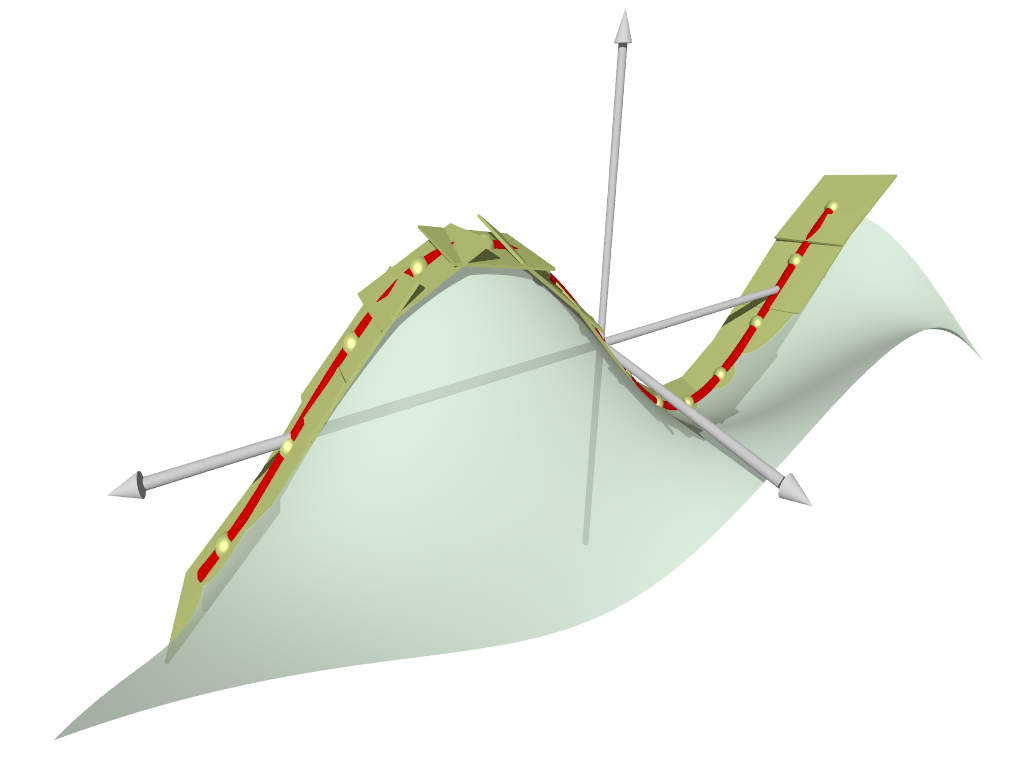
\includegraphics[width=\hsize]{../common/3d/streifen0.png}
\caption{A strip consists of the values and tangent planes
along a curve (red).
The green surface is a solution of the wave equation with the
data of the strip as initial data.
\label{skript:streifen}}
\end{figure}

\begin{figure}
\centering
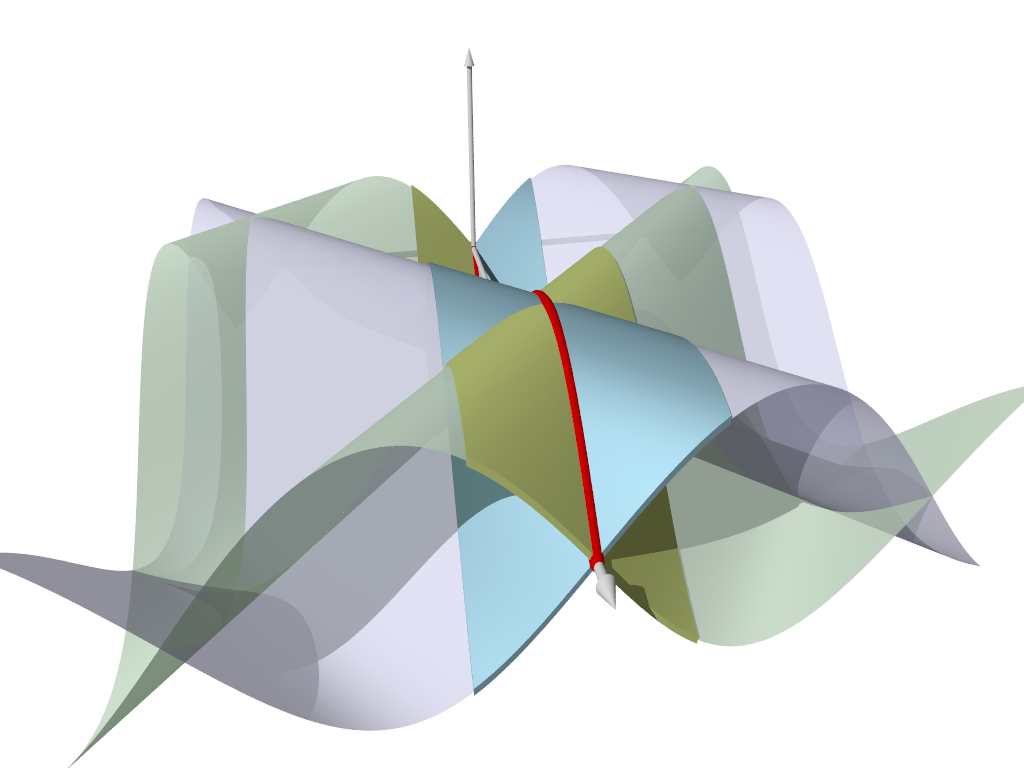
\includegraphics[width=\hsize]{../common/3d/streifen2.png}
\caption{Along the common red curve both solution surfaces have
the same initial values, but different tangent planes, so they
have different strips.
\label{skript:streifen:eindeutig}}
\end{figure}

\begin{figure}
\centering
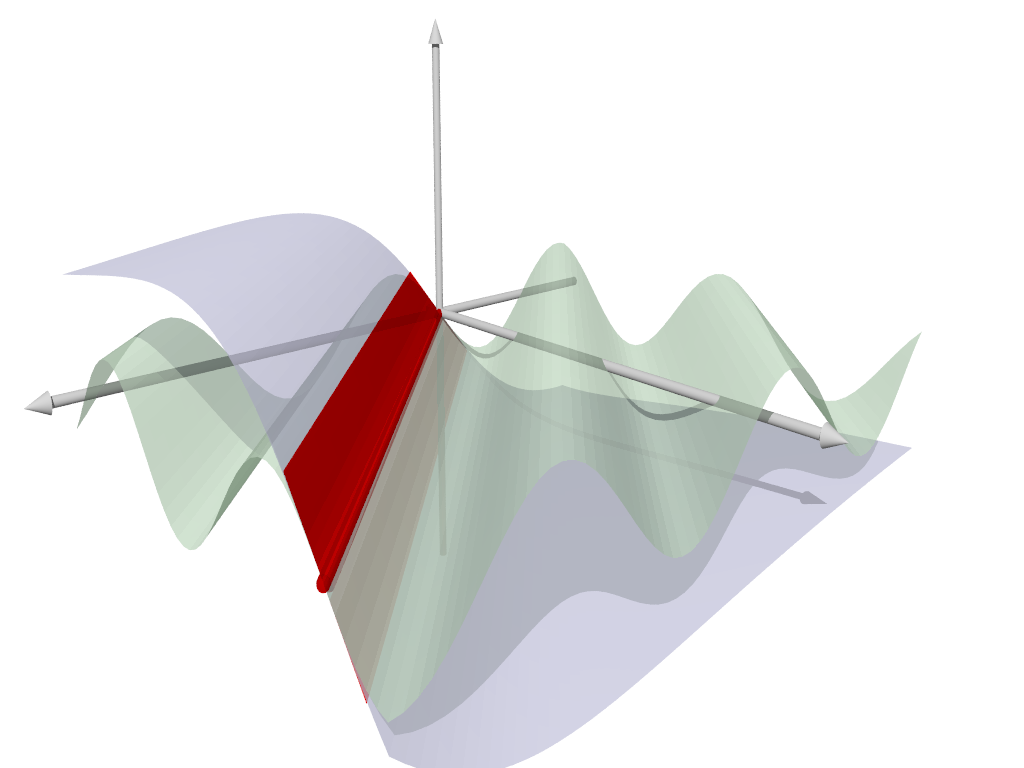
\includegraphics[width=\hsize]{../common/3d/streifen1.png}
\caption{Characteristics are those curves that cannot be used to
define a strip that would uniquely determine the solution surface.
The graph shows two solution of the wave equation with the same
strip: they go through the same curve and they have the same
tangent planes, but the differ in the curvature perpendicular to the
initial curve.
This means that the second order derivatives are not determined by
the equation and the strip data.
\label{skript:streifen:zweideutig}}
\end{figure}

The functions $u(t)$, $p(t)$ and $q(t)$ are not completely arbitrary.
By deriving the first equation \eqref{charanfangs} with respect to $t$,
we find
\[
\dot{u}(t)=\frac{d}{dt}u(t)
=
\frac{d}{dt}u(x(t),y(t))
=
\frac{\partial u}{\partial x}(x(t), y(t))\frac{d}{dt}x(t)
+
\frac{\partial u}{\partial y}(x(t), y(t))\frac{d}{dt}y(t).
\]
Since the partial derivatives are also given in \eqref{charanfangs},
we must also have the relation
\begin{equation}
\dot{u}(t)= p(t)\dot{x}(t) + q(t)\dot{y}(t).
\label{cauchydatarestriction}
\end{equation}

\subsection{Characteristic curves\label{subsection:characteristics-curves}}
Specifying the data of a strip often determines the hyperbolic
partial differential equation uniquely.
In figure~\ref{skript:streifen:eindeutig} two different solutions
are shown that have the same initial curve but different tangent
planes, so the have different strips along this curve.

Deriving the last two equations of \eqref{charanfangs} with respect to $t$,
gives the system of linear equations
\[
\begin{linsys}{3}
\dot p(t)
&=&
\partial_x\partial_xu(x(t),y(t))\,\dot x(t)
&+&
\partial_x\partial_yu(x(t),y(t))\,\dot y(t)
& &
\\
\dot q(t)
&=&
& &
\partial_x\partial_yu(x(t),y(t))\,\dot x(t)
&+&
\partial_y\partial_yu(x(t),y(t))\,\dot y(t)
\end{linsys}
\]
Together with the differential equation we have now three linear equations
to determine the second partial derivatives (colored red)
\[
\begin{linsys}{4}
a{\color{red}\displaystyle\frac{\partial^2 u}{\partial x^2}}
&+&
2b{\color{red}\displaystyle\frac{\partial^2 u}{\partial x\partial y}}
&+&
c{\color{red}\displaystyle\frac{\partial^2 u}{\partial y^2}}
&=&
h(t)\phantom{.}
&=&
g-dp(t)-eq(t)-fu\\
\dot x(t)
{\color{red}\displaystyle\frac{\partial^2 u}{\partial x^2}}
&+&
\dot y(t)
{\color{red}\displaystyle\frac{\partial^2 u}{\partial x\partial y}}
& &
&=&
\dot p(t)\phantom{.}
& &
\\
& &
\dot x(t)
{\color{red}\displaystyle\frac{\partial^2 u}{\partial x\partial y}}
&+&
\dot y(t)
{\color{red}\displaystyle\frac{\partial^2 u}{\partial y^2}}
&=&
\dot q(t).
& &
\end{linsys}
\]
This linear system of equations for the second order derivatives
has the coefficient matrix
\[
\begin{pmatrix}
a&2b&c\\
\dot x(t)&\dot y(t)&0\\
0&\dot x(t)&\dot y(t)
\end{pmatrix}.
\]
The system of equation is not or not uniquely solvable if the
determinant vanishes, i.~e.
\begin{align*}
0&=\left|\begin{matrix}
a&2b&c\\
\dot x(t)&\dot y(t)&0\\
0&\dot x(t)&\dot y(t)
\end{matrix}\right|
\\
&=a\dot y(t)^2-2b\dot x(t)\dot y(t)+c\dot x(t)^2
\end{align*}

\begin{definition}
The characteristics of a differential equation of the form
\eqref{charequation}
are the curves
$t\mapsto(x(t),y(t))$, for which the initial data 
\eqref{charanfangs} does not determine the second partial
derivatives uniquely.
\end{definition}

\begin{satz}
\label{charakteristikendgl}
The characteristics of a partial differential equation
\eqref{charequation}
solve the differential equation
\[
a\dot y(t)^2-2b\dot x(t)\dot y(t)+c\dot x(t)^2=0.
\]
\end{satz}

\subsection{Characteristic strip}
We shoose a characteristic $t\mapsto(x(t),y(t))$.
We are only interested in the case where there are infinitely
many possible values for the second derivative.
This case happens when the determinants
\[
\left|
\begin{matrix}
h&2b&c\\
\dot p(t)&\dot y(t)&0\\
\dot q(t)&\dot x(t)&\dot y(t)
\end{matrix}
\right|
,
\quad
\left|
\begin{matrix}
a&h&c\\
\dot x(t)&\dot p(t)&0\\
0&\dot q(t)&\dot y(t)
\end{matrix}
\right|
,
\quad
\left|
\begin{matrix}
a&2b&h\\
\dot x(t)&\dot y(t)&\dot p(t)\\
0&\dot x(t)&\dot q(t)
\end{matrix}
\right|
\]
all vanish, where $h=g-dp(t)-eq(t)-fu(x(t),y(t))$.
It suffices the select a single one of those determinants,
we choose the second:
\begin{align*}
a\dot p(t)\dot y(t)-h\dot x(t)\dot y(t)+c\dot x(t)\dot q(t)&=0
\end{align*}

Together with the condition~\eqref{cauchydatarestriction}
we now have three equations that the functions
$x$, $y$, $u$, $p$ and $q$ must satisfy in order for the second
derivatives to not be determined uniquely by the initial data.

\begin{definition}
A strip along a characteristic which satisfies
\[
a\dot p(t)\dot y(t)-h\dot x(t)\dot y(t)+c\dot x(t)\dot q(t)=0
\]
is called a {\em characteristic strip}.
\end{definition}

Thus it is also possible that the integral surfaces of a partial
differential equation touch along a curve, but are different
nevertheless.
By necessity, the tangent planes along the intersection curve form
a characteristic strip.

\begin{satz}
\label{skript:satz:charakteristiken}
If two different integral surfaces touch along a curve,
then this curve together with the tangent planes form a characteristic strip.
\end{satz}

Figure~\ref{skript:streifen:zweideutig} shows two solutions of the wave
equation that touch along a characteristic.
From theorem~\ref{skript:satz:charakteristiken} the red strip is a 
characteristic strip.

\begin{proof}
Apparently there are at least two different solutions of the
partial differential equation that contain the curve which in
addition have the same tangent planes.
The curve and the tangent planes do not determine the solution
uniquely, so they form a characteristic strip.
\end{proof}

\subsection{Examples}
\subsubsection{Wave equation}
The characteristics of the wave equation
\begin{equation}
\partial_t^2u-a^2\partial_x^2u=0
\label{hyperbolisch:wellengleichung}
\end{equation}
are the curves $s\mapsto(t(s),x(s))$, that satisify the equation
\begin{align*}
\left(
\frac{dx(s)}{ds}\right)^2-a^2\left(\frac{dt(s)}{ds}\right)^2&=0
\\
\frac{dx(s)}{ds}
&=
\pm a\frac{dt(s)}{ds}
\\
\Rightarrow
\frac{dx}{dt}=\pm a.
\end{align*}
These are straight lines with slope $\pm a$.
\begin{figure}
\centering
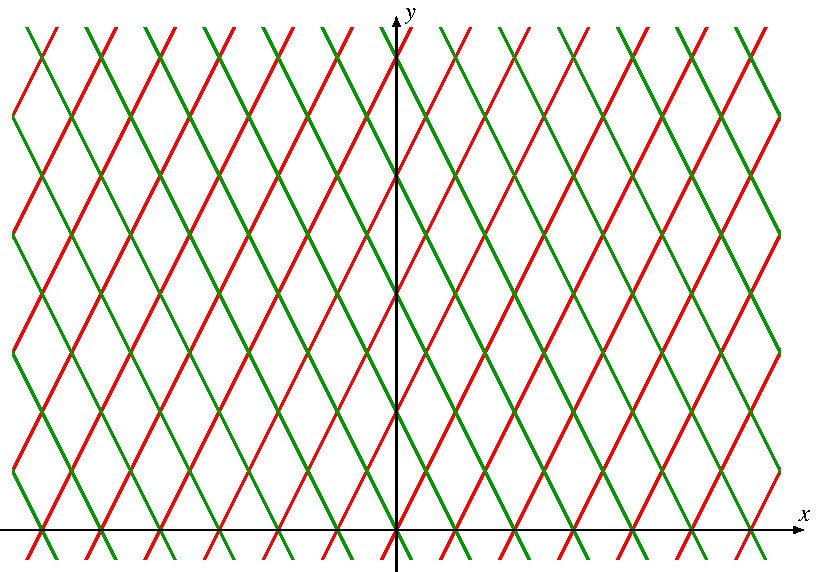
\includegraphics{9-hyperbolic/images/wavechar.pdf}
\caption{Characteristics of the wave
equation~(\ref{hyperbolisch:wellengleichung})
\label{hyp:wellen}}
\end{figure}
Figure~\ref{hyp:wellen} shows the characteristics.

\subsubsection{The equation $\partial_x\partial_yu=0$}
The condition for the characteristics in this case is
\[
-\dot x(t)\dot y(t)=0
\]
One of the derivatives must disappear, which is only possible for
curves that are parallel to the $x$- or the $y$-axis.
Figure~\ref{hyp:dxdy} shows these characteristics
\begin{figure}
\centering
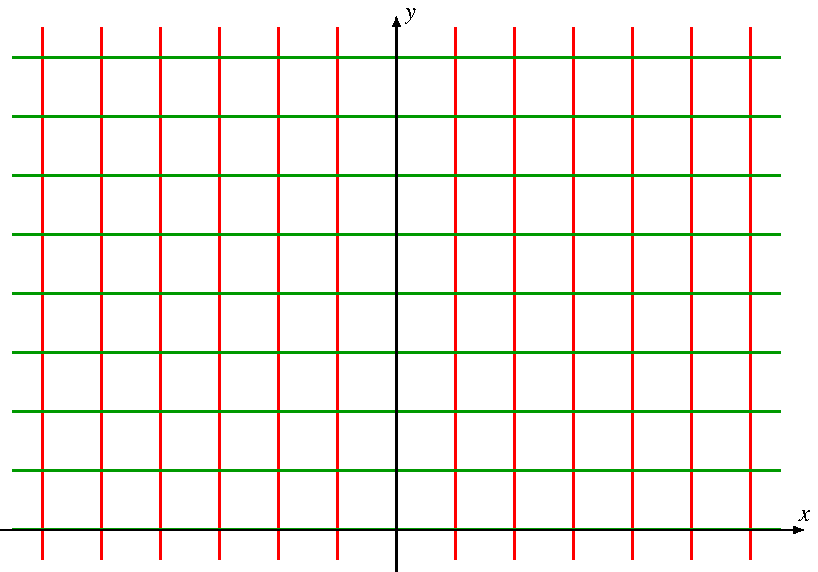
\includegraphics{9-hyperbolic/images/dxdy.pdf}
\caption{characteristics of the hyperbolic partial differential equation
$\partial_x\partial_yu=0$.
\label{hyp:dxdy}}
\end{figure}

\subsubsection{Curved characteristics}
The partial differential equation
\begin{equation}
\partial_t^2u-x^2\partial_x^2u=0
\label{hyperbolisch:gekruemmt}
\end{equation}
is hyperbolic for $x\ne 0$.
The characteristics satisfy the equation
\begin{align*}
x'(s)^2-x^2t'(s)^2&=0
\\
xt'&=\pm  x'
\\
\frac{d}{ds}t&=\pm\frac{d}{ds}\log x
\\
t&=\pm\log x+C
\\
x&=x_0e^{\pm t}
\end{align*}
The characteristics are exponential curves.
In figure \ref{hyp:exp}
the characteristics for the positive sign are drawn in red,
the characteristics for the negative sign green.
\begin{figure}
\centering
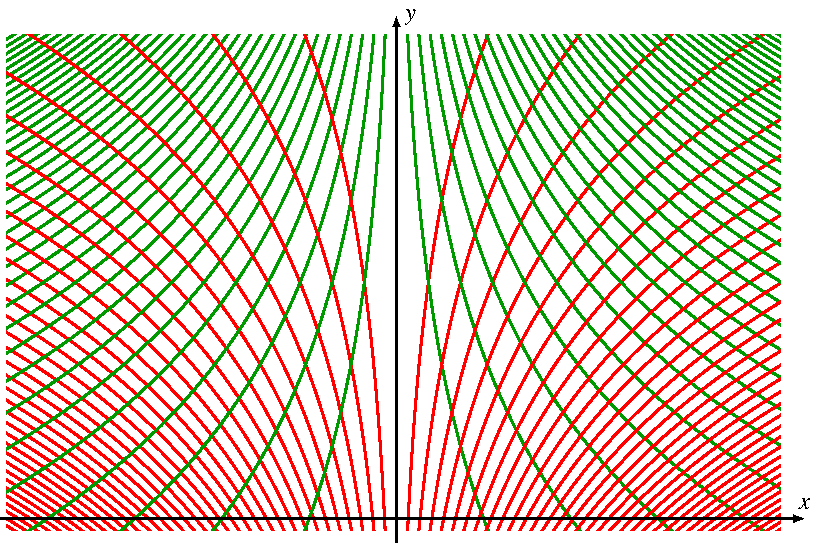
\includegraphics{9-hyperbolic/images/exponential.pdf}
\caption{Characteristics for $x\ne 0$ for the hyperbolic partial
differential equation~\eqref{hyperbolisch:gekruemmt}.
\label{hyp:exp}}
\end{figure}

This equation describes a wave equation in a medium in which
the wave velocity increases with increasing $x$.
The exponential curves suggest that the wave becomes faster when moving ``out''.

\subsection{Characteristics of elliptic or parabolic partial differential
equations}
The theory of the characteristics developed above can also be
applied to elliptic or hyperbolic partial differential equations.

In the elliptic case, the differential equation of the characteristics
\[
a\dot y(t)^2-2b\dot x(t)\dot y(t)+c\dot x(t)^2=0
\]
does not have any solutions, as the expression only vanishes only for
$\dot x(t)=0$ and $\dot y(t)=0$.

For parabolic partial differential equations the characteristic
equation becomes in a suitable coordinate system
\[
-\kappa t'(s)^2=0.
\]
This can only hold true if $t$ is constant.
The characteristics in this case are straight lines parallel
to the $x$-axis.
In fact it is not possible to determine the second derivative
with respect to $t$ for initial data along a line parallel
to the $x$-axis.

We will summarize the information about causality or which points on
the boundery can influence the solution in which points of the domain
in section~\ref{section:which-boundary-points}

\subsection{Some interesting theorems}

\begin{satz}
Every integral surface can be covered with a set of characteristic
strips.
\end{satz}

\begin{proof}
Let $u$ be the solution of a partial differential equation.
The differential equation in theorem~\ref{charakteristikendgl}
describes two curves $t\mapsto(x(t),y(t))$ in every point of the domain.
Obviously it is possible to cover the solution surface by such curves.
By substituting these curves into $u(x,y)$, $\partial_xu(x,y)$
and $\partial_yu(x,y)$ we get a set of characteristic strips
as claimed.
\end{proof}

\begin{satz}
If a set of characteristic strips covers a surface $S$ defined
by the function $u(x,y)$ and this function has continuous 
second derivatives then $u$ is a solution of the differential equation.
\end{satz}

\begin{proof}
The characteristic strips satisfy the equations
\begin{equation}
\begin{gathered}
a\dot y(t)^2-2b\dot x(t)\dot y(t)+c\dot x(t)^2=0,
\\
a\dot p(t)\dot y(t)-h\dot x(t)\dot y(t)+c\dot x(t)\dot q(t)=0,
\\
\dot u(t)=p(t)\dot x(t)+q(t)\dot y(t).
\end{gathered}
\label{alle}
\end{equation}
Let's call the second derivatives of $u$ along a cahracteristic curve
\begin{align*}
R&=\partial_x^2u(x(t),y(t)),
\\
S&=\partial_x\partial_yu(x(t),y(t)),
\\
T&=\partial_y^2u(x(t),y(t)).
\end{align*}
We can write
\begin{align*}
\dot p(t)&=R(t)\dot x(t)+S(t)\dot y(t)\qquad\text{and}\\
\dot q(t)&=S(t)\dot x(t)+T(t)\dot y(t).
\end{align*}
If we substitute this in the second equation of \eqref{alle}, we get
\begin{align*}
a(R\dot x+S\dot y)\dot y-h\dot x\dot y+c\dot x(S\dot x+T\dot y)&=0
\\
\Rightarrow \qquad(aR-h+cT)\dot x\dot y+aS\dot y^2 +cS \dot x^2&=0.
\end{align*}
Multiplying the first equation of
\eqref{alle} by $t$ and subtracting it we get
\[
(aR+2bS+cT-h)\dot x\dot y=0.
\]
Writing out the parenthesis leads to the equation
\[
a\partial_x^2u+2b\partial_x\partial_yu+c\partial_y^2u-h=0
\]
which is the original differential equation.
\end{proof}
This theorem teaches that the hyperbolic partial differential equation
can be solved by looking for characteristic strips.
for this it suffices the solve ordinary differential equations for the
functions $x$, $y$, $p$, $q$, $R$, $S$ and $T$.



%
% discontinuities.tex -- 
%
% (c) 2019 Prof Dr Andreas Mueller
%
\section{Propagation of discontinuities}
\rhead{Discontinuities}
The study of the wave equation at the beginning of this chapter
allowed us to find solutions as translates of an initial function
$u_0$ along the characteristics, which were straight lines
$x\pm at=\operatorname{const}$.
If $u_0$ is not everywhere differentiable, then the solution will
not be differentiable along the characteristic.

Assume that $u$ is continuously differentiable everywhere
and twice continuously differentiable everywhere
except along a curve.
This curve separates the domain into subdomains.
In each subdomain, $u$ is a solution of the differential equation
with the same boundary values and tangent planes on the curve.
This implies that the curve and the tangent planes must
specify a characteristic strip.

\begin{satz}
If $u$ is continuously differentiable everywhere and twice
continuously differentiable everywhere except along a curve,
and $u$ is a solution everywhere except on that curve,
then that curve is a characteristic.
\end{satz}

This means that discontinuities of the second derivative
can only propagate along the characteristic curves.

The wave equation can be used to approximately compute the
flow around a supersonic plane.
The plane produces shock waves which are discontinuities in the
solution of the wave equation.
According to the theorem above, these shock waves follow
characteristic curves.
The can be made visible using the Schlieren technique
(figure~\ref{ueberschall2d}).

\begin{figure}
\begin{center}
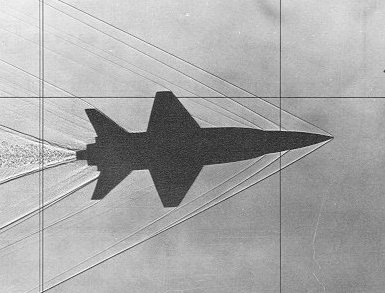
\includegraphics[width=0.8\hsize]{../common/graphics/i-5-1}
\end{center}
\caption{Flow around a supersonic plane\label{ueberschall2d}}
\end{figure}


%
% higherdim.tex -- XXX
%
% (c) 2019 Prof Dr Andreas Mueller
%
\section{Charakteristiken in höheren Dimensionen}
\rhead{Charakteristiken in höheren Dimensionen}
Wir wollen jetzt die Frage nach den Charakteristiken in höheren Dimensionen
stellen. Um die Diskussion überschaubar zu halten, beschränken wir uns auf
das dreidimensionale Problem. Die gefundenen Schlussfolgerungen 
lassen sich sofort auf beliebig viele Dimensionen verallgemeinern.

\subsection{Problemstellung}
Das Cauchy-Problem für eine partielle Differentialgleichung der
Form
\[
\sum_{i,j=1}^3a_{ij}\partial_i\partial_ju+\sum_{i=1}^3b_i\partial_iu+cu=f
\]
besteht darin, dass auf einer Fläche, die zum Beispiel durch
eine Gleichung
\[
\omega(x_1,x_2,x_3)=0
\]
gegeben werden kann,
die Funktionswerte von $u$ vorgegeben werden, sowie die ersten
Ableitungen in eine Richtung senkrecht auf die Fläche.
Diese Ableitung kann mit Hilfe des Gradienten berechnet werden:
\[
\frac{\partial u}{\partial n}=\operatorname{grad}u\cdot \frac{\operatorname{grad}\omega}{|\operatorname{grad}\omega|}
\]
Die Lösung hängt wieder davon ab, ob die Differentialgleichung
und die Anfangsbedingungen die zweiten Ableitungen von $u$ bereits
eindeutig bestimmen.

\subsection{Ein Spezialfall}
Wir betrachten wieder den Spezialfall, in dem die Anfangswerte auf der
Ebene $x_1=0$ vorgegeben sind, also
\begin{align*}
u(0,x_2,x_3)&=u_0(x_2,x_3),
\\
\partial_1u(0,x_2,x_3)&=h(x_2,x_3)
\end{align*}
Dies entspricht dem Fall $\omega(x_1,x_2,x_3)=x_1$.

Durch die Vorgabe der Anfangswerte in Form der Funktion $u_0$ sind die Ableitungen
$\partial_iu$ für $i=2,3$ ebenfalls festgelegt.
Durch Ableiten der Anfangsbedingungen nach $x_2,\dots,x_3$
sind auch die zweiten Ableitungen 
\[
\partial_i\partial_ju(0,x_2,x_3)\qquad 2\le i\le 3,\;1\le j\le 3
\]
bekannt. Es ist also nur noch $\partial_1^2u$ zu bestimmen.
Die Differentialgleichung kann nach $\partial_1^2u$ aufgelöst
werden, wenn $a_{11}\ne 0$. Dies ist gleichbedeutend damit, dass
\[
a_{11}=\begin{pmatrix}
1&0&\dots&0
\end{pmatrix}
A
\begin{pmatrix}1\\0\\\vdots\\0\end{pmatrix}
=0.
\]

\subsection{Der allgemeine Fall}
Wir betrachten die Funktion $\omega(x_1,x_2,x_3)$ als die erste
Koordinaten eines neuen Koordinatensystems. Die Koordinaten in diesem
neuen System nennen wir $\omega_1,\dots,\omega_3$, sie sind Funktionen
der alten Koordinaten
\[
\omega_1(x_1,x_2,x_3)=\omega(x_1,x_2,x_3)
,\qquad
\omega_2(x_1,x_2,x_3)
,\qquad
\omega_3(x_1,x_2,x_3)
\]
Die Funktion $u$ kann natürlich auch in den neuen Koordinaten geschrieben
werden: $\tilde u(\omega_1,\omega_2,\omega_3)$ hat die Eigenschaft
\[
\tilde u(
\omega_1(x_1,x_2,x_3),
\omega_2(x_1,x_2,x_3),
\omega_3(x_1,x_2,x_3)) = u(x_1,x_2,x_3).
\]
Setzt man dies in die Differentialgleichung ein, ergibt sich
\begin{align*}
\partial_iu
&=
\sum_{k=1}^3
\frac{\partial\tilde u}{\partial \omega_k}
\frac{\partial\omega_k}{\partial x_i}
\\
\partial_i\partial_ju
&=
\sum_{k,l=1}^3
\frac{\partial^2\tilde u}{\partial \omega_k\partial\omega_l}
\frac{\partial\omega_k}{\partial x_i}
\frac{\partial\omega_l}{\partial x_j}
\\
\sum_{i,j=1}^3a_{ij}\partial_i\partial_ju
&=
\sum_{i,j,k,l=1}^3a_{ij}
\frac{\partial^2\tilde u}{\partial \omega_k\partial\omega_l}
\frac{\partial\omega_k}{\partial x_i}
\frac{\partial\omega_l}{\partial x_j}
\\
\sum_{i=1}^3b_i\partial_iu
&=
\sum_{i,k=1}^3b_i
\frac{\partial\tilde u}{\partial \omega_k}
\frac{\partial\omega_k}{\partial x_i},
\end{align*}
die Differentialgleichung für $\tilde u$ in den neuen 
Koordinaten lautet also
\[
\sum_{k,l=1}^3a_{ij}
\biggl(
\sum_{i,j=1}^3a_{ij}
\frac{\partial\omega_k}{\partial x_i}
\frac{\partial\omega_l}{\partial x_j}
\biggr)
\frac{\partial^2\tilde u}{\partial \omega_k\partial\omega_l}
+
\sum_{k=1}^3
\biggl(
\sum_{i=1}^3
b_i
\frac{\partial\omega_k}{\partial x_i}
\biggr)
\frac{\partial\tilde u}{\partial \omega_k}
+c\tilde u
=f.
\]
Die neuen Koeffizienten der zweiten Ableitungen sind also
\[
\tilde a_{kl}=
\sum_{i,j=1}^3a_{ij}
\frac{\partial\omega_k}{\partial x_i}
\frac{\partial\omega_l}{\partial x_j}
\]
Die Fläche entspricht in den $\omega$-Koordinaten dem Spezialfall $\omega_1=0$,
die zweiten Ableitungen sind also genau dann eindeutig bestimmt, wenn
der Koeffizient $\tilde a_{11}$ nicht verschwindet. Entlang der durch $\omega$
definierten Fläche sind also genau dann die zweiten Ableitungen nicht eindeutig
bestimmt, wenn 
\[
\sum_{i,j=1}^3
a_{ij}
\frac{\partial\omega}{\partial x_i}
\frac{\partial\omega}{\partial x_j}
=
\operatorname{grad}\omega
\cdot
A
\operatorname{grad}\omega
=0
\]
Da der Gradient senkrecht auf der Fläche steht, also alle Flächen
problematisch, deren Normalen $\vec n$ die Vektorgleichung
\[
\vec n\cdot A\vec n=0
\]
erfüllen. Diese Vektoren heissen {\em charakteristische Normalen}.

\begin{definition}
Eine durch $\omega(x_1,\dots,x_n)=0$ definierte Fläche heisst
charakteristische Fläche, wenn auf der Fläche
\[
\sum_{i,j=1}^na_{ij}\partial_i\omega\partial_j\omega=0
\]
gilt.
\end{definition}

\subsection{Charakteristische Flächen der Wellengleichung}
\begin{figure}
\begin{center}
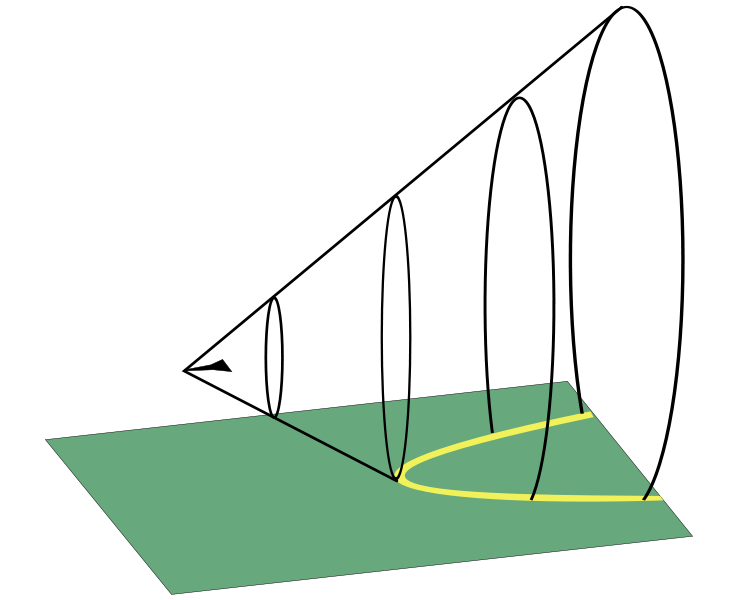
\includegraphics[width=0.8\hsize]{../common/graphics/shock}
\end{center}
\caption{Schockwelle eines Überschallflugzeugs als Beispiel einer
charakteristischen Fläche von $\partial_t^2u-a^2\Delta u=0$.\label{ueberschallkegel}}
\end{figure}
Wir bestimmen die charakteristischen Flächen der
Wellengleichung
\[
\partial_t^2u-a^2\Delta u=0.
\]
Die Koeffizientenmatrix ist
\[
\begin{pmatrix}
1&0&0\\
0&-a^2&0\\
0&0&-a^2
\end{pmatrix},
\]
die charakteristischen Normalen sind also Vektoren $\vec v$, welche die
Gleichung
\[
v_1^2-a^2v_2^2-a^2v_3^2=0
\]
erfüllen. Diese beschreibt einen Doppelkegel, alle Vektoren, welche mit
der $x_1$-Achse einen festen Winkel einschliessen, sind charakteristische
Normalen. Der Winkel $\alpha$ muss der Bedingung
\[
\cos^2\alpha-a^2\sin^2\alpha=0
\]
genügen, also
\[
\tan\alpha=\pm\frac1a.
\]

Die Winkelbedingung ist die einzige Einschränkung an
die charakteristischen Flächen,  entsprechend gibt es eine
grosse Vielfalt:
\begin{enumerate}
\item
Jeder Kegel mit halbem Öffnungswinkel $\frac{\pi}2-\alpha$
und Achse parallel zur $x_1$-Achse ist eine charakteristische Fläche.
Der Kegel schneidet cie $x_2$-$x_3$-Ebene in einem Kreis, dessen Radius mit
grösser werdendem $x_1$ mit der Geschwindigkeit $a$ grösser wird.

Abbildung \ref{ueberschallkegel}
zeigt die Schockwelle eines Überschallflugzeuges. Schockwellen
als Unstetigkeiten müssen sich entlang der charakteristischen Flächen ausbreiten,
also entlang eines Kegels.
\item 
Jede Ebene, die mit der $x_1$-Achse einen Winkel von $\frac\pi2-\alpha$
einschliesst, ist charakteristische Fläche.
Die Ebene schneidet die $x_2$-$x_3$-Ebene in einer Geraden, die sich
mit der Geschwindigkeit $a$ senkrecht zur Geraden fortbewegt.
Diese charakteristische Fläche beschreibt die Fortpflanzung einer
ebenen Welle.
\end{enumerate}



%
% boundry.tex  -- 
%
% (c) 2019 Prof Dr Andreas Mueller
%
\section{Boundary conditions}
The method of characteristics allows us to find out on which parts of the
boundary we have to specify boundary conditions to make the solution
unique.
The solution surface corresponding to $u(x,y)$ consists of characteristics
so it is uniquely determined if exactly one characteristic goes through
each point.

For the differential equation
\begin{equation}
\frac{\partial u}{\partial x}+2\frac{\partial u}{\partial y}=3
\label{geometrie:knickbeispiel}
\end{equation}
we have found the characteristics
\[
t\mapsto\begin{pmatrix}x_0\\y_0\\z_0\end{pmatrix}+t\begin{pmatrix}1\\2\\3\end{pmatrix}.
\]
The graph of the solution function $u(x,y)$ must be covered by characteristics.
The projections of these curves into the $x$-$y$-plane are straight lines
with slope $2$.
The boundary of the domain $\Omega$, in which the equation needs to be
solved, thus must intersect each straight line with slope $2$ exactly once.

The domain
$\{(x,y)\in\mathbb R^2\,|\, x >0\}$  from \ref{konstantekoeff}
has the $x$-axis as boundary which intersects every straight line with
slope exactly once.

The domain $\Omega=\{(x,y)\,|\,0<x,y<1\}$ is more interesting.
Figures \ref{geometrie:charrand1}
to \ref{geometrie:charrand3}
show various possibilities:
\begin{enumerate}
\item
In figure~\ref{geometrie:charrand1}
boundary values are prescribed on the left and right boundary.
These boundary values are not sufficient to determine the solution
everywhere in the domain.
There is a part not covered by characteristics where the solution
is not fixed.
\item
In figure~\ref{geometrie:charrand2}
boundary values are given on the top and bottom boundaries of the
square.
A solution is only possible if the values solution emanating from
the left half of the bottom boundary coincides with the solution
emanating from the right half of the top boundary.
If the boundary values on these parts are not compatible, no solution
exists.
\item
In figure~\ref{geometrie:charrand3}
the boundary values are specified on the left and bottom side
of the square.
This fixes the solution function uniquely.
Nevertheless it is not entirely clear that we have found a solution,
because it is still possible that the combined function is not
differentiable on the characteristic through the lower left
corner of the square.
\end{enumerate}
The last situation is very common, the solution we find here is
differentiable outside of a set of measure zero.
This is called a {\em weak} solution of the differential equation.

\begin{figure}
\begin{center}
\includegraphics{../common/images/randwerte-2.pdf}
\end{center}
\caption{Boundary values on the left and right side: solution
not determined in the light green portion of the domain.
\label{geometrie:charrand1}}
\end{figure}

\begin{figure}
\begin{center}
\includegraphics{../common/images/randwerte-3.pdf}
\end{center}
\caption{Boundary values on the top and bottom side of the square:
solution overdetermined in the light green portioin of the domain
\label{geometrie:charrand2}}
\end{figure}

\begin{figure}
\begin{center}
\includegraphics{../common/images/randwerte-4.pdf}
\end{center}
\caption{Boundary values on the left and bottom sides of the square:
solution well defined but differentiability on the light green
characteristic emanating from $(0,0)$ is not guaranteed.
\label{geometrie:charrand3}}
\end{figure}

\begin{figure}
\centering
\includegraphics[width=\hsize]{../common/3d/knick.jpg}
\caption{The solution of the differential
equation~(\ref{geometrie:knickbeispiel}),
with boundary values along the left and bottom sides of the square
(see also figure~\ref{geometrie:charrand3})
is not differentiable along the characteristic through $(0,0)$
(vertical axis scaled by a factor $0.4$).
\label{geometrie:knick}}
\end{figure}

As an illustration of the last case consider the boundary values
\begin{align*}
u(x_0,0)&=0,\\
u(0,y_0)&=y_0.
\end{align*}
Each side fixes part of the solution in the unit square, we can get 
explicit formulas using the method of characteristics.
The characteristics starting from the bottom side are
\[
\left.
\begin{aligned}
x&=x_0+t\\
y&=2t\\
u&=3t
\end{aligned}
\right\}
\qquad\Rightarrow\qquad
\left\{
\begin{aligned}
t&=\frac12y\\
u&=\frac32y
\end{aligned}
\right.
\]
The characteristics from the left side of the square are
\[
\left.
\begin{aligned}
x&=t\\
y&=y_0+2t\\
u&=y_0+3t
\end{aligned}
\right\}
\qquad\Rightarrow\qquad
\left\{
\begin{aligned}
y_0&=y-2x\\
u&=y+x
\end{aligned}
\right.
\]
Thus the solution function is
\[
u(x,y)=\begin{cases}
\frac32y&\qquad y<2x\\
x+y&\qquad y>2x,
\end{cases}
\]
as displayed in figure~\ref{geometrie:knick}.
For $y=2x$, both terms coincide, so the solution function is continuous
in all of $\Omega$.
However, the partial function $x\mapsto u(x,y)$ has slope $1$
for $y>2x$ and slope $0$ for $y<2x$, so it is not differentiable at $y=2x$.



\section{Zusammenfassung: das Wichtigste in Kürze}
\begin{enumerate}
\item Jede Lösungsfläche einer hyperbolischen partiellen Differentialgleichung
kann mit charakteristischen Streifen überdeckt werden.
\item Unstetigkeiten breiten sich entlang von Charakteristiken aus.
\item Wie bei quasilinearen partiellen Differentialgleichungen erster
Ordnung kann mit Hilfe der Charakteristiken abgeschätzt werden, wo
Randwerte und Ableitungen vorgegeben werden müssen, damit ein hyperbolisches
Problem gut gestellt ist.
\end{enumerate}

